% ======================================================================
%  CampusSwap: final-stage project report (UCS503P)
%
%  Build on Overleaf: upload this whole folder, set the compiler to
%  pdfLaTeX (XeLaTeX also works) and the bibliography tool to biber.
%  The files in generated/ are written by
%      python project-report-final/tools/make_test_tables.py
%  from a real pytest run. Do not edit them by hand.
% ======================================================================
\documentclass{tietreport}

% Fonts: Latin Modern on both pdfLaTeX and XeLaTeX
\usepackage{iftex}
\ifPDFTeX
  \usepackage[T1]{fontenc}
  \usepackage[utf8]{inputenc}
  \usepackage{lmodern}
\else
  \usepackage{fontspec}
\fi

% Images
\usepackage{graphicx}
\graphicspath{{figures/}}

% Tables, lists, floats, algorithm
\usepackage{booktabs}
\usepackage{tabularx}
\usepackage{array}
\usepackage{longtable}
\usepackage{xltabular}
\usepackage{pdflscape}
\usepackage{float}
\usepackage{enumitem}
\usepackage{subcaption}
\usepackage{algorithm}
\usepackage{algpseudocode}
\usepackage{xcolor}
\usepackage{xurl}
% Lets long test names break after an underscore (no hyphen is added)
\usepackage[nohyphen]{underscore}

% Bibliography configuration (as in the TIET template)
\usepackage[
  date=year,
  style=alphabetic,
  backend=biber,
  sorting=nty,
  maxnames=5,
  minnames=3,
  maxalphanames=4,
  minalphanames=3,
  backref=true,
  doi=false,
  isbn=false,
  url=true,
  eprint=false
]{biblatex}
\addbibresource{references.bib}

% Numbers from the last real test run: \TestsTotal, \TestsPassed,
% \TestsFailed, \TestsSeconds, \TestsDate, \CasesTotal
\newcommand{\TestsTotal}{175}
\newcommand{\TestsPassed}{175}
\newcommand{\TestsFailed}{0}
\newcommand{\TestsSeconds}{40.6}
\newcommand{\TestsDate}{03 November 2026}
\newcommand{\CasesTotal}{48}


\setlength{\headheight}{15pt}
\setlist{itemsep=2pt}
\newcolumntype{L}[1]{>{\raggedright\arraybackslash}p{#1}}
\newcolumntype{Y}{>{\raggedright\arraybackslash}X}
\hypersetup{colorlinks=true, linkcolor=black, citecolor=blue!50!black, urlcolor=blue!50!black}

% A screenshot that may not exist yet. If the file is missing, a framed
% placeholder is printed instead, so the document still compiles.
%   \screenshot[max height]{file name in figures/}{width}
\newcommand{\screenshot}[3][0.8\textheight]{%
  \IfFileExists{figures/#2}%
    {\includegraphics[width=#3,height=#1,keepaspectratio]{#2}}%
    {\fbox{\parbox[c][3cm][c]{\dimexpr #3-2\fboxsep-2\fboxrule\relax}%
      {\centering\small missing: \texttt{#2}}}}%
}

% Requirement status
\newcommand{\Built}{Built}
\newcommand{\Planned}{\textbf{Planned}}
\newcommand{\Req}[1]{\texttt{#1}}

% Reads a file of table rows. TeX's own \input primitive is used because
% it is expandable, so a file whose first row starts with \multicolumn
% still works inside a table.
\makeatletter
\newcommand{\InputRows}[1]{\@@input #1 }
\makeatother

% Used by the test-case table (see Chapter 5)
\newlength{\AutoByWidth}
\let\OrigMulticolumn\multicolumn
\newcommand{\AutoByMulticolumn}[3]{%
  \OrigMulticolumn{#1}{@{}>{\raggedright\arraybackslash}p{\AutoByWidth}@{}}{#3}}

%% ==================================================
%% TITLE PAGE
%% ==================================================

\TitlePageHeader{%
  UCS503P Software Engineering Lab: Project Report%
}

\ProjectTitle{%
  CampusSwap%
}

\ProjectSubTitle{%
  Room-Exchange and Slot-Coordination System for Campus\\[0.2cm]
  Final-stage report: multi-way hostel room swaps and
  lecture slot swaps with Top Trading Cycles%
}

\author{%
  \texttt{1024240152} Jahnavi \\
  \texttt{1024240102} Ronit Saini \\
  \texttt{1024240001} Ranvir \\
  \texttt{1024240010} Krishna Kapoor%
}

\TitlePageSubText{%
  BE Third Year, 2026--27%
}

\AdvisorName{%
  Dr. Raghav B. Venkataramaiyer%
}

\TitlePageFooterText{{%
    \large Final Evaluation \\[0.2cm]
    \bfseries Computer Science and Engineering
    Department%
  } \\[0.15cm]
  Thapar Institute of Engineering and Technology,
  Patiala%
}

%% ==================================================

\begin{document}

\maketitle

\tableofcontents
\listoffigures
\listoftables

% =====================================================
\chapter{Introduction}
\label{ch:intro}
% =====================================================

\section{Background and Motivation}

Hostel rooms at a university are given out once, at the start of a
semester, and are then rarely changed. Students who would like to move,
for example to a lower floor, a single room, or closer to friends, can
only do so by \emph{trading} with another student, because the hostels
are close to full. Today these trades are arranged through WhatsApp
groups, notice boards and personal contacts, and the hostel office
approves them on paper.

Teachers have the same problem with their weekly timetable. A lecture
slot (a fixed day, time and lecture hall) may suit one teacher badly and
another teacher well, but there is no simple way for them to find each
other and agree a swap.

\textbf{CampusSwap} turns both of these into one software workflow.
Each person says what they have (a bed, or a lecture slot) and ranks up
to five things they would prefer. The system finds \emph{chains} of
exchanges in which every member moves to something they ranked; every
member confirms; and the hostel office approves. The matching step uses
the \textbf{Top Trading Cycles} (TTC) algorithm of Shapley and
Scarf~\cite{shapley1974cores}, the standard method for markets in which
each participant already owns one item that cannot be split, such as a
room~\cite{abdulkadiroglu1999house}.

\section{Problem Statement}

The current process has four weak points, identified in our proposal:

\begin{itemize}
  \item \textbf{Scattered information:} requests are spread over chat
    groups and notice boards, so open offers are hard to find.
  \item \textbf{Only direct swaps are found:} people look for a partner
    who wants exactly their room (A with B). Chains such as
    A~$\rightarrow$~B~$\rightarrow$~C~$\rightarrow$~A satisfy everyone
    without an empty room, but are almost impossible to find by hand.
  \item \textbf{Paperwork:} approved swaps need paper applications, and
    there is no central record.
  \item \textbf{No visibility:} people cannot tell whether their request
    is waiting, matched, or impossible.
\end{itemize}

\section{Users}

\begin{itemize}
  \item \textbf{Students} who live in a hostel. They browse rooms, rank
    rooms (or room types), confirm or decline a proposed chain, and
    follow their request on a dashboard.
  \item \textbf{Hostel staff} (the warden's office). They run matching
    rounds by hand or on a timetable, approve confirmed chains, download
    the approval form and the records, and run lecture-slot rounds.
  \item \textbf{Faculty} (teachers). They offer one of their lecture
    slots, rank slots they would prefer, and confirm or decline a
    proposed slot swap.
\end{itemize}

\section{Objectives}

The prototype stage met objectives O1--O5 of the proposal (data model,
student module, matching engine, dashboards, evaluation on synthetic
data). For the final stage the objectives were to build every
requirement that the Software Requirements Specification (SRS) still
marked \emph{Planned}:

\begin{enumerate}
  \item \textbf{F1 -- Safer sign-in:} only institute addresses, limits
    on repeated wrong passwords, and an HTTPS-only mode.
  \item \textbf{F2 -- Better requests:} rank a \emph{type} of room (for
    example ``any single AC room on floor~1'') instead of one room.
  \item \textbf{F3 -- Less manual work:} email notices and reminders,
    matching rounds on a timetable, a printable approval form (PDF), and
    a download of the full event log.
  \item \textbf{F4 -- Faculty slot exchange:} the second half of the
    project title, using the same matching engine.
  \item \textbf{F5 -- Evidence:} a test case for every requirement that
    can be tested automatically, with results taken from a real test run.
\end{enumerate}

\section{What Was Built Since the Prototype}

\begin{table}[H]
\centering
\small
\begin{tabularx}{\textwidth}{@{}lY@{}}
\toprule
\textbf{Feature} & \textbf{What it does} \\
\midrule
Institute email only & The server itself refuses any address that does not end in \texttt{@thapar.edu}. \\
Sign-in limits & Too many wrong passwords within 15 minutes block further tries for a while. \\
HTTPS mode & When switched on, plain web addresses are redirected to secure ones and the login cookie is only sent over a secure connection. \\
Room-type choices & A choice can be ``any room of this kind in this hostel''. \\
Email outbox and reminders & Every chain member gets a ``match found'' email and, if they have not answered, one reminder 12 hours before the deadline. \\
Automatic rounds & Staff can set a round to run every $N$ hours. \\
Approval form & A one-page PDF for each approved swap, with signature lines. \\
Event log download & The whole audit trail as a spreadsheet file (CSV). \\
Faculty slot exchange & A new \emph{Faculty} role, a new page for teachers and a \emph{Slots} tab for staff. \\
One active request, enforced by the database & Two quick clicks on \emph{Submit} can no longer create two requests. \\
\bottomrule
\end{tabularx}
\caption{Features added in the final stage.}
\label{tab:new}
\end{table}

Only one requirement is still not built: \Req{FR-AUTH-11}, sign-in with
the institute's Microsoft account. Section~\ref{sec:sso} explains why.
All data in the system and in this report is made up.

% =====================================================
\chapter{Requirements}
\label{ch:req}
% =====================================================

\section{Where the Requirements Come From}

The requirements are written in the team's SRS (\texttt{srs/main.tex},
version~1.1). Each has an identifier: \texttt{FR} for a
\emph{functional} requirement (something the system does) and
\texttt{NFR} for a \emph{non-functional} requirement (how well or how
safely it does it). The SRS also lists eleven business rules
(\texttt{BR-01} to \texttt{BR-11}); they are covered by the functional
requirements below and are not repeated here.

\section{Requirement Status}

Table~\ref{tab:status} lists every requirement. The last column says how
it is checked:
\begin{itemize}
  \item \textbf{TC-xx} is an automated test case in Table~\ref{tab:testcases}
    (Chapter~\ref{ch:test}).
  \item \textbf{HC-xx} is a check done by hand on the page
    (Table~\ref{tab:handchecks}), for behaviour that only exists in the
    browser.
  \item A test name in \texttt{typewriter} font is an automated test
    listed in Appendix~\ref{app:tests} that is not part of a test case.
  \item \textbf{No test} means the rule is in the code but nothing checks
    it automatically. We say so rather than hide it.
\end{itemize}

{\small
\setlength{\tabcolsep}{4pt}
\begin{xltabular}{\textwidth}{@{}l Y l L{3.9cm}@{}}
\caption{Every requirement, its status and how it is checked.}\label{tab:status}\\
\toprule
\textbf{ID} & \textbf{Requirement (short)} & \textbf{Status} & \textbf{Checked by} \\
\midrule
\endfirsthead
\multicolumn{4}{@{}l}{\itshape Table~\ref{tab:status} continued}\\
\toprule
\textbf{ID} & \textbf{Requirement (short)} & \textbf{Status} & \textbf{Checked by} \\
\midrule
\endhead
\midrule
\multicolumn{4}{@{}r}{\itshape continued on the next page}\\
\endfoot
\bottomrule
\endlastfoot
\multicolumn{4}{@{}l}{\textbf{Sign in and sessions}}\\
\Req{FR-AUTH-01} & Sign in with email, password and role (Student, Hostel Staff, Faculty) & \Built & TC-01, TC-03 \\
\Req{FR-AUTH-02} & Ignore letter case and spaces in the email & \Built & TC-06 (capitals accepted) \\
\Req{FR-AUTH-03} & Same answer for an unknown email and a wrong password & \Built & TC-02 \\
\Req{FR-AUTH-04} & Right password on the wrong tab: say which tab to use & \Built & TC-03 \\
\Req{FR-AUTH-05} & 12-hour session in the \texttt{cs\_session} cookie & \Built & TC-01 \\
\Req{FR-AUTH-06} & Sign out deletes the session & \Built & TC-04 \\
\Req{FR-AUTH-07} & Every action needs a signed-in user of the right role & \Built & TC-05 \\
\Req{FR-AUTH-08} & The sign-in page accepts only \texttt{@thapar.edu} & \Built & HC-05 \\
\Req{FR-AUTH-09} & The server also refuses other addresses & \Built & TC-06 \\
\Req{FR-AUTH-10} & Slow down or block repeated failed sign-ins & \Built & TC-07, TC-08, TC-09, TC-10 \\
\Req{FR-AUTH-11} & Sign in with the institute's Microsoft account & \Planned & -- (Section~\ref{sec:sso}) \\
\midrule
\multicolumn{4}{@{}l}{\textbf{Browse rooms}}\\
\Req{FR-ROOM-01} & Show only rooms in hostels of the student's gender & \Built & TC-13 \\
\Req{FR-ROOM-02} & Show hostel, block, floor, number, beds, AC, washroom, tags & \Built & by hand on the page \\
\Req{FR-ROOM-03} & Show how many occupants want to swap, without names & \Built & by hand on the page \\
\Req{FR-ROOM-04} & Mark the student's own room; it cannot be ranked & \Built & TC-16 (server refuses it); marking by hand \\
\Req{FR-ROOM-05} & Filters and search & \Built & by hand on the page \\
\Req{FR-ROOM-06} & Detailed and compact views, in pages & \Built & by hand on the page \\
\Req{FR-ROOM-07} & Rank a room type instead of one room & \Built & TC-19, TC-20, TC-21 \\
\midrule
\multicolumn{4}{@{}l}{\textbf{Submit and withdraw a request}}\\
\Req{FR-REQ-01} & Rank one to five rooms and submit them & \Built & TC-14, TC-38 \\
\Req{FR-REQ-02} & Reorder by dragging or with buttons; remove & \Built & HC-03 \\
\Req{FR-REQ-03} & Refuse empty list, more than five, duplicates & \Built & TC-15 \\
\Req{FR-REQ-04} & Refuse a student with no seat or an active request & \Built & TC-16, TC-17 \\
\Req{FR-REQ-05} & Refuse unknown room, own room, other gender's hostel & \Built & TC-16 \\
\Req{FR-REQ-06} & Save as \emph{open} with a tracking ID \texttt{CS-YYYY-NNNN} & \Built & TC-14 \\
\Req{FR-REQ-07} & Withdraw only while open & \Built & TC-18 \\
\Req{FR-REQ-08} & Record every submit and withdraw in the event log & \Built & TC-14, TC-41 (submit is logged); withdraw: no test \\
\midrule
\multicolumn{4}{@{}l}{\textbf{Run a matching round}}\\
\Req{FR-MATCH-01} & Staff run a TTC round over every open request & \Built & TC-22, TC-38 \\
\Req{FR-MATCH-02} & Dissolve overdue chains before building the pool & \Built & TC-32 (dissolving); that a round does it first: no test \\
\Req{FR-MATCH-03} & Offer the beds of a shared room in a fixed order & \Built & \texttt{test\_double\_room\_seats\_are\_tried\_in\_listed\_order} \\
\Req{FR-MATCH-04} & Never assign an unranked room & \Built & TC-21, TC-23, TC-24 \\
\Req{FR-MATCH-05} & A saved round creates proposed chains with a 48-hour deadline & \Built & TC-22 \\
\Req{FR-MATCH-06} & A dry run changes nothing & \Built & TC-25 \\
\Req{FR-MATCH-07} & Report pool size, matched, Match Yield, chain lengths, trace & \Built & TC-26 \\
\Req{FR-MATCH-08} & Only one round at a time (\texttt{409 run\_in\_progress}) & \Built & no test \\
\Req{FR-MATCH-09} & Compare TTC with direct 1:1 swaps; 1:1 only as a dry run & \Built & TC-27 \\
\Req{FR-MATCH-10} & Rounds run automatically on a timetable & \Built & TC-29 \\
\midrule
\multicolumn{4}{@{}l}{\textbf{Accept or decline a chain}}\\
\Req{FR-CONF-01} & Show each member the whole chain & \Built & HC-04 \\
\Req{FR-CONF-02} & Accept once; all accepted means \emph{confirmed} & \Built & TC-30, TC-38 \\
\Req{FR-CONF-03} & One decline dissolves the chain & \Built & TC-31 \\
\Req{FR-CONF-04} & A chain past its deadline is dissolved & \Built & TC-32 \\
\Req{FR-CONF-05} & Refuse answers from outsiders, late or repeated answers & \Built & TC-32, TC-33 \\
\Req{FR-CONF-06} & Email each member when a chain is found and before the deadline & \Built & TC-34, TC-35 \\
\midrule
\multicolumn{4}{@{}l}{\textbf{Approve a chain}}\\
\Req{FR-APPR-01} & Approve only a chain every member accepted & \Built & TC-36 \\
\Req{FR-APPR-02} & On approval everyone moves, in one transaction & \Built & TC-36, TC-38 \\
\Req{FR-APPR-03} & A signed-off approval form (PDF) & \Built & TC-37 \\
\midrule
\multicolumn{4}{@{}l}{\textbf{Status tracking and reports}}\\
\Req{FR-TRACK-01} & Dashboard: room, request, chain, five milestones & \Built & TC-39 \\
\Req{FR-TRACK-02} & Dashboard: last 20 events, newest first & \Built & TC-39 (newest first) \\
\Req{FR-TRACK-03} & Dashboard explains the next step & \Built & TC-39 \\
\Req{FR-TRACK-04} & Staff overview numbers & \Built & TC-40 \\
\Req{FR-TRACK-05} & Staff request table & \Built & TC-40 \\
\Req{FR-TRACK-06} & Requests as \texttt{campusswap-requests.csv} & \Built & TC-41 \\
\Req{FR-TRACK-07} & Public numbers on the sign-in page & \Built & TC-42 \\
\Req{FR-TRACK-08} & Download the full event log & \Built & TC-41 \\
\midrule
\multicolumn{4}{@{}l}{\textbf{Faculty slot exchange}}\\
\Req{FR-SLOT-01} & Faculty rank lecture slots; the same engine finds slot chains & \Built & TC-43 to TC-47, HC-06 \\
\midrule
\multicolumn{4}{@{}l}{\textbf{Performance}}\\
\Req{NFR-PERF-01} & 2{,}000 requests matched in under 2 seconds & \Built & TC-28 \\
\Req{NFR-PERF-02} & Time grows at most with the square of the pool size & \Built & argument in Section~\ref{sec:ttc} \\
\Req{NFR-PERF-03} & Usable on a 390-pixel-wide phone screen & \Built & HC-01 \\
\Req{NFR-PERF-04} & Works with no internet access & \Built & HC-02 \\
\midrule
\multicolumn{4}{@{}l}{\textbf{Safety}}\\
\Req{NFR-SAFE-01} & Every change in one database transaction & \Built & TC-36 \\
\Req{NFR-SAFE-02} & The database allows one occupant per seat & \Built & no test (unique rule in \texttt{models.py}) \\
\Req{NFR-SAFE-03} & The database rejects rows that point at nothing & \Built & no test (switched on in \texttt{db.py}) \\
\Req{NFR-SAFE-04} & No room or rank twice in one request (database rules) & \Built & TC-17 \\
\Req{NFR-SAFE-05} & Only made-up data & \Built & TC-48 \\
\Req{NFR-SAFE-06} & No student names while browsing rooms & \Built & TC-13 \\
\midrule
\multicolumn{4}{@{}l}{\textbf{Security}}\\
\Req{NFR-SEC-01} & Salted \emph{scrypt} password hashes & \Built & TC-12 \\
\Req{NFR-SEC-02} & 32-byte session tokens; only their hash stored & \Built & TC-12 \\
\Req{NFR-SEC-03} & Cookie HttpOnly, SameSite=Lax, 12 hours & \Built & TC-01 (cookie set); the flags: no test \\
\Req{NFR-SEC-04} & Role checked on the server for every request & \Built & TC-05 \\
\Req{NFR-SEC-05} & User text escaped before it is shown & \Built & by hand on the page \\
\Req{NFR-SEC-06} & Errors do not reveal whether an account exists & \Built & TC-02 \\
\Req{NFR-SEC-07} & Deployed site only over HTTPS, cookie Secure & \Built & TC-11 \\
\Req{NFR-SEC-08} & Limit repeated failed sign-ins & \Built & TC-07 \\
\end{xltabular}
}

\paragraph{Summary.} Of the 72 requirements (54 functional, 18 non-functional), 71 are built and one
(\Req{FR-AUTH-11}) is planned. Six built requirements have no automated
check of the exact rule: \Req{FR-REQ-08} (for withdrawals),
\Req{FR-MATCH-02} (the order of steps in a round), \Req{FR-MATCH-08},
\Req{NFR-SAFE-02}, \Req{NFR-SAFE-03} and the cookie flags of
\Req{NFR-SEC-03}. For each, the rule can be read in the named file, but a
test would be needed to prove it keeps working.

\section{Microsoft Single Sign-On (FR-AUTH-11)}
\label{sec:sso}

\emph{Single sign-on} means a student signs in with the Microsoft account
the institute already gives them, instead of a separate CampusSwap
password. To do this, CampusSwap must be registered as an application
inside Thapar's own Microsoft account system (its \emph{tenant}). The
registration gives the application an ID and a secret, and tells
Microsoft which web address to send users back to after they sign
in~\cite{msregister}. Only the institute's IT office can create that
registration; the team cannot. Without it, the sign-in flow cannot be
built against the real service or tested from start to end, and a version
that was never run would break the rule that the report only claims what
the code does. The requirement therefore stays \emph{Planned}. Until it
is built, users sign in with their institute email address and a password,
protected by the limits described in Section~\ref{sec:signin}.

% =====================================================
\chapter{Design}
\label{ch:design}
% =====================================================

\section{Use Cases}

Figure~\ref{fig:usecase} shows the use cases of students and hostel
staff. The faculty use cases are the same steps applied to lecture slots:
\emph{offer a slot and rank others}, \emph{withdraw}, \emph{confirm or
decline a slot swap}; staff add \emph{run a slot round} and \emph{approve a
slot swap}. Staff also gained \emph{set the round timetable},
\emph{download the approval form} and \emph{download the event log}.

\begin{figure}[H]
  \centering
  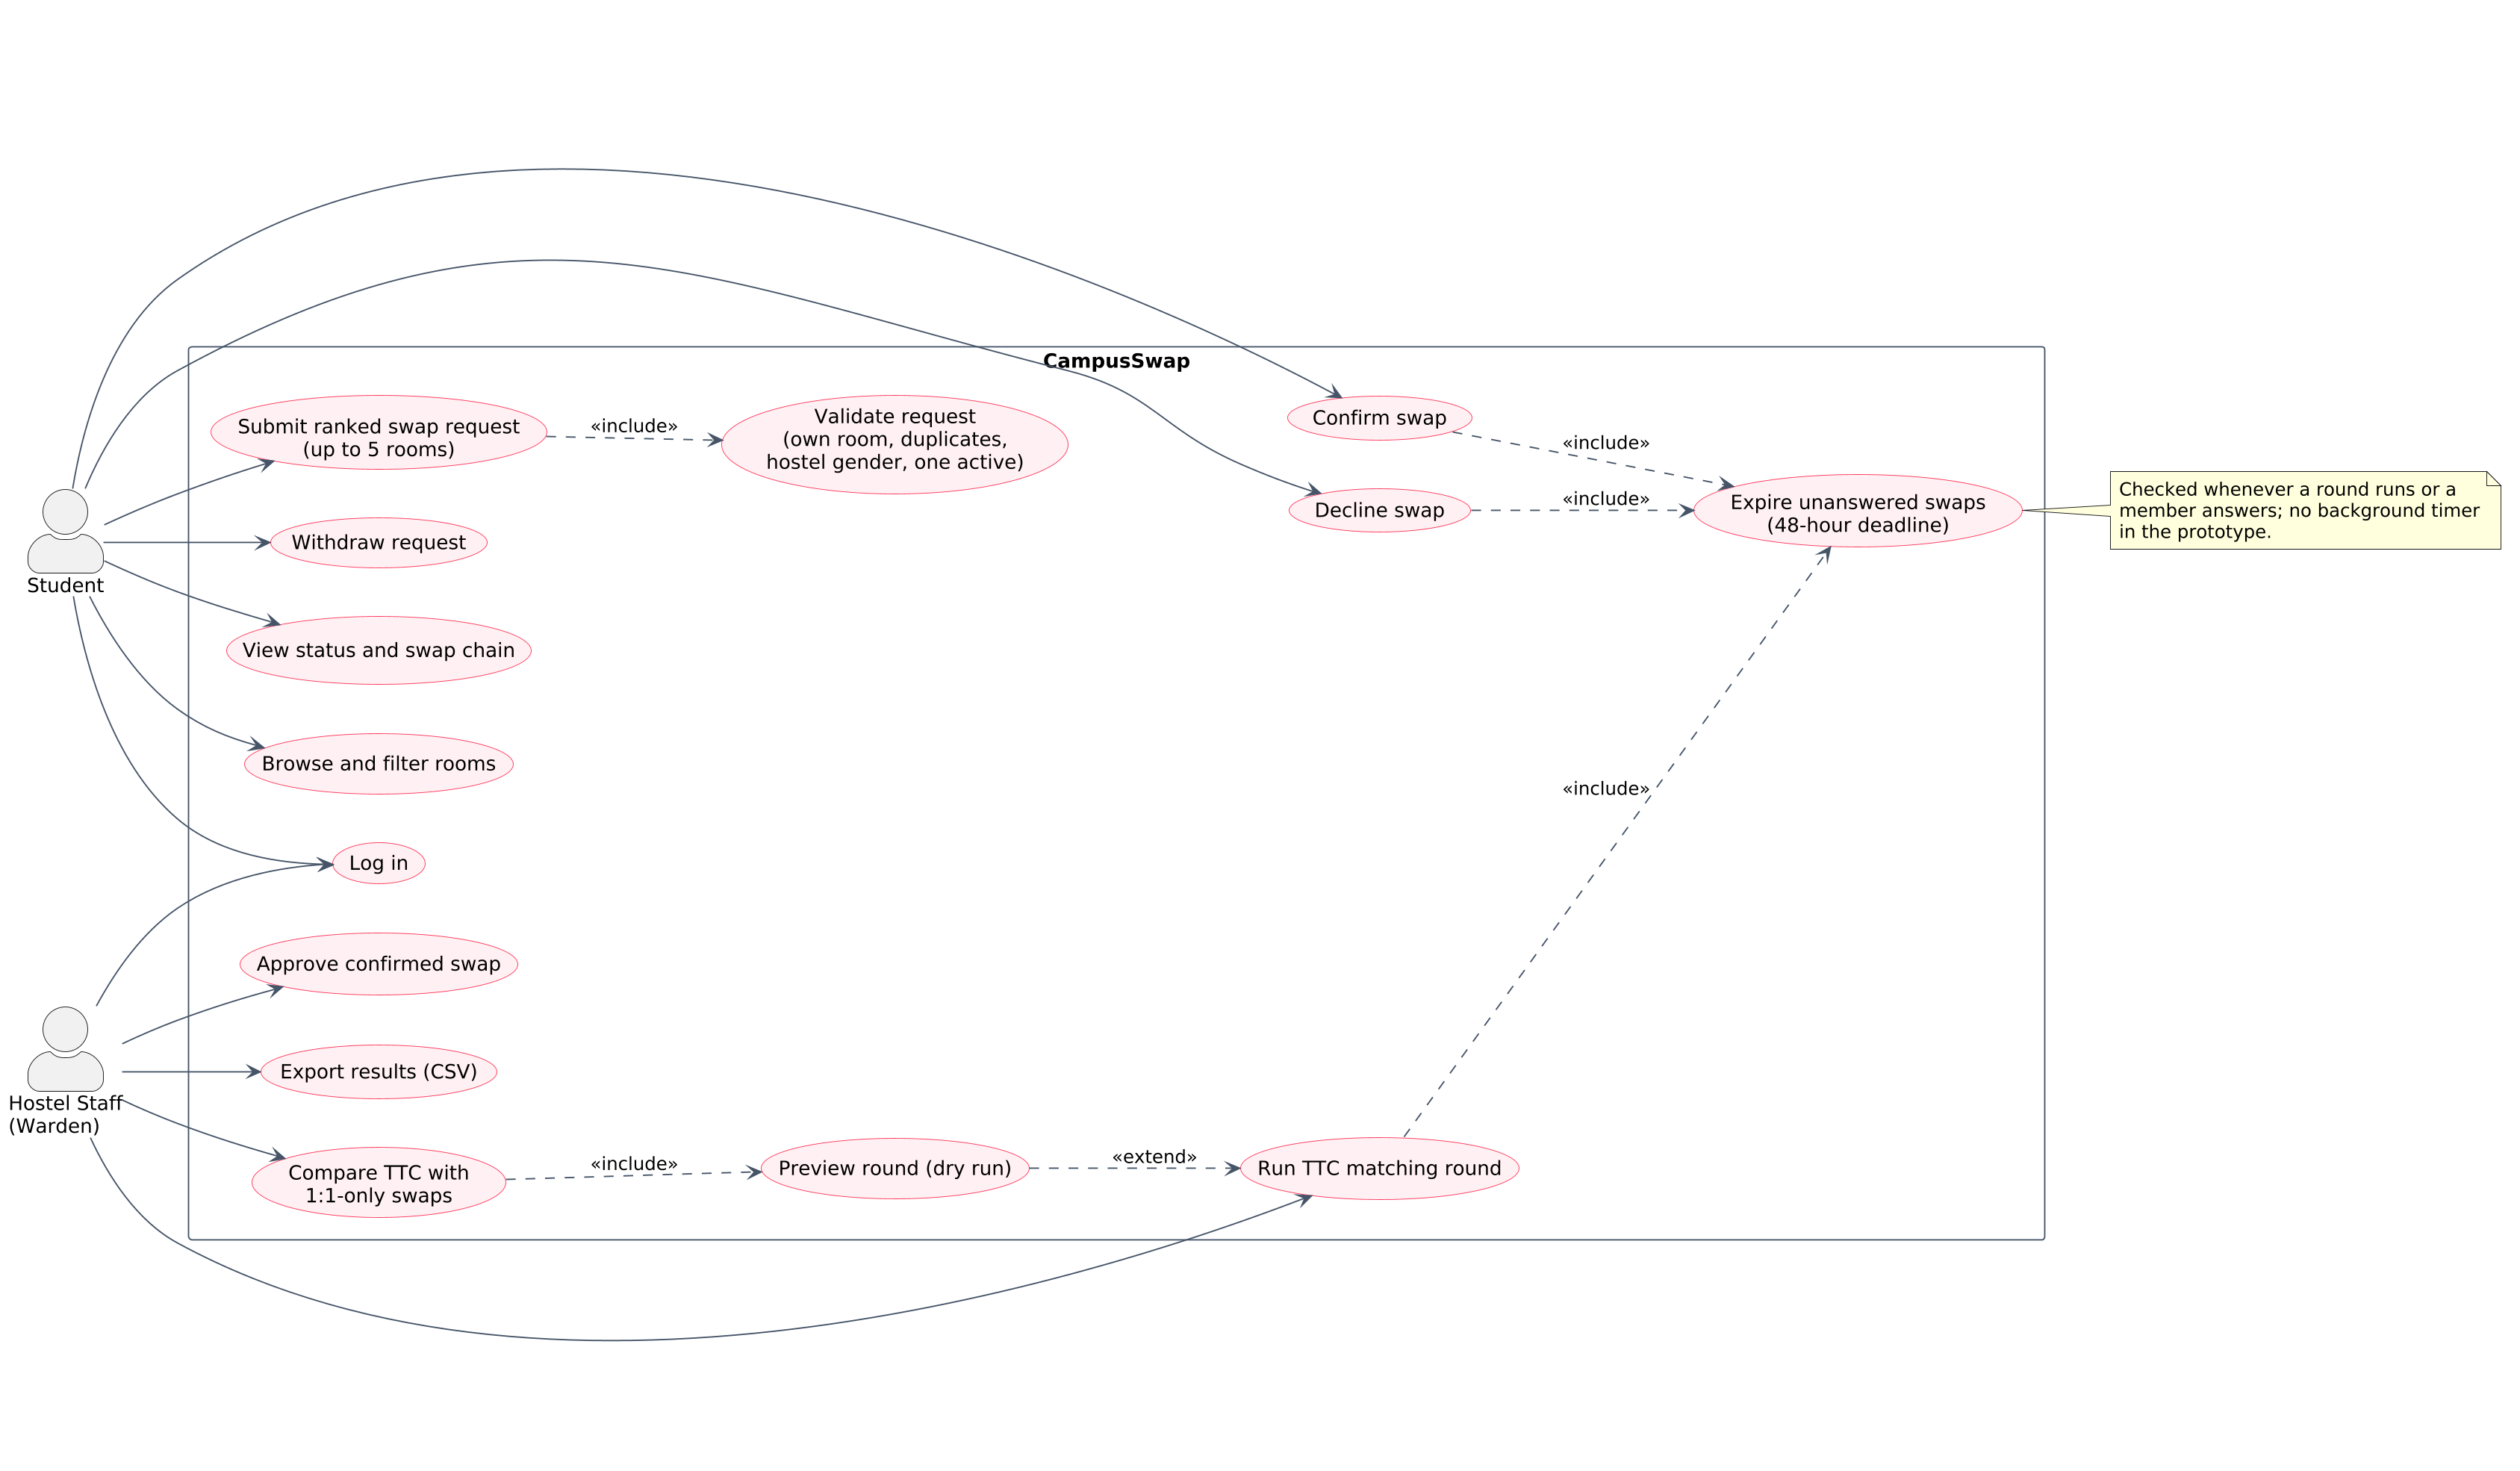
\includegraphics[width=\textwidth,height=0.75\textheight,keepaspectratio]{use-case.png}
  \caption[Use case diagram]{Use case diagram. It was drawn at the
    prototype stage: it has no Faculty actor and does not show the
    final-stage use cases listed in the text above.}
  \label{fig:usecase}
\end{figure}

\section{System Architecture}

CampusSwap is a web application in three layers, plus a separate
matching engine (Figure~\ref{fig:arch}).

\begin{enumerate}
  \item \textbf{Pages} (what users see): five HTML pages (sign-in, rooms,
    student dashboard, staff console, faculty slots), each with a small
    JavaScript file. The pages talk to the server through an \emph{API}
    (a set of web addresses under \texttt{/api} that send and receive data
    as \emph{JSON}, a plain-text data format).
  \item \textbf{Server}: \emph{routes} written with FastAPI~\cite{fastapi}
    check who is signed in and their role, then call a \emph{service}.
    The services (\texttt{app/services/}) hold every business rule. A route
    never contains a rule.
  \item \textbf{Data}: an SQLite database file, used through
    SQLAlchemy~\cite{sqlalchemy}, a library that maps Python classes to
    database tables.
  \item \textbf{Engine} (\texttt{code/backend/engine/}): Top Trading Cycles,
    the 1:1 comparison and the Match Yield measure, in plain Python with no
    database or web code. The room service and the slot service both call
    the same engine.
\end{enumerate}

\begin{figure}[H]
  \centering
  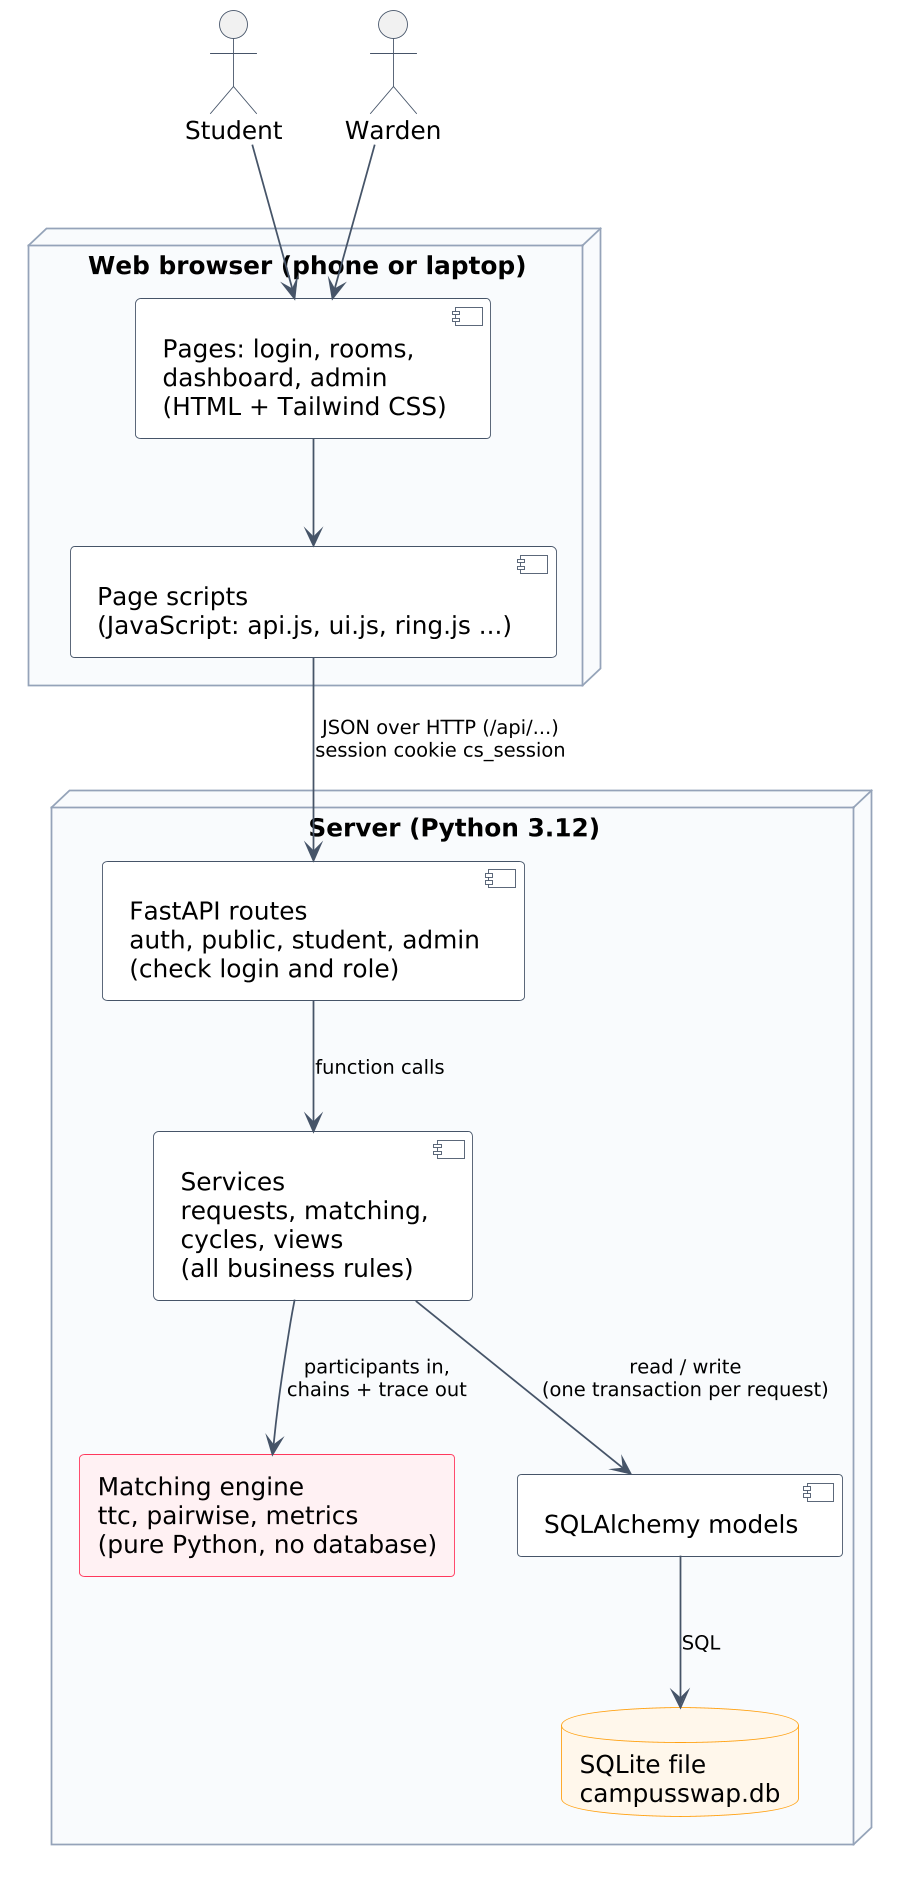
\includegraphics[width=\textwidth,height=0.7\textheight,keepaspectratio]{architecture.png}
  \caption[Architecture]{Architecture. Drawn at the prototype stage: it
    does not show the faculty routes and page, the new services
    (\texttt{signin}, \texttt{mail}, \texttt{schedule}, \texttt{pdf},
    \texttt{slots}), the background check or the mail server. They sit in
    the same layers as the parts shown.}
  \label{fig:arch}
\end{figure}

The data flow diagrams (Figures~\ref{fig:dfd0} and~\ref{fig:dfd1}) show
what information moves between users, processes and stored data.

\begin{figure}[H]
  \centering
  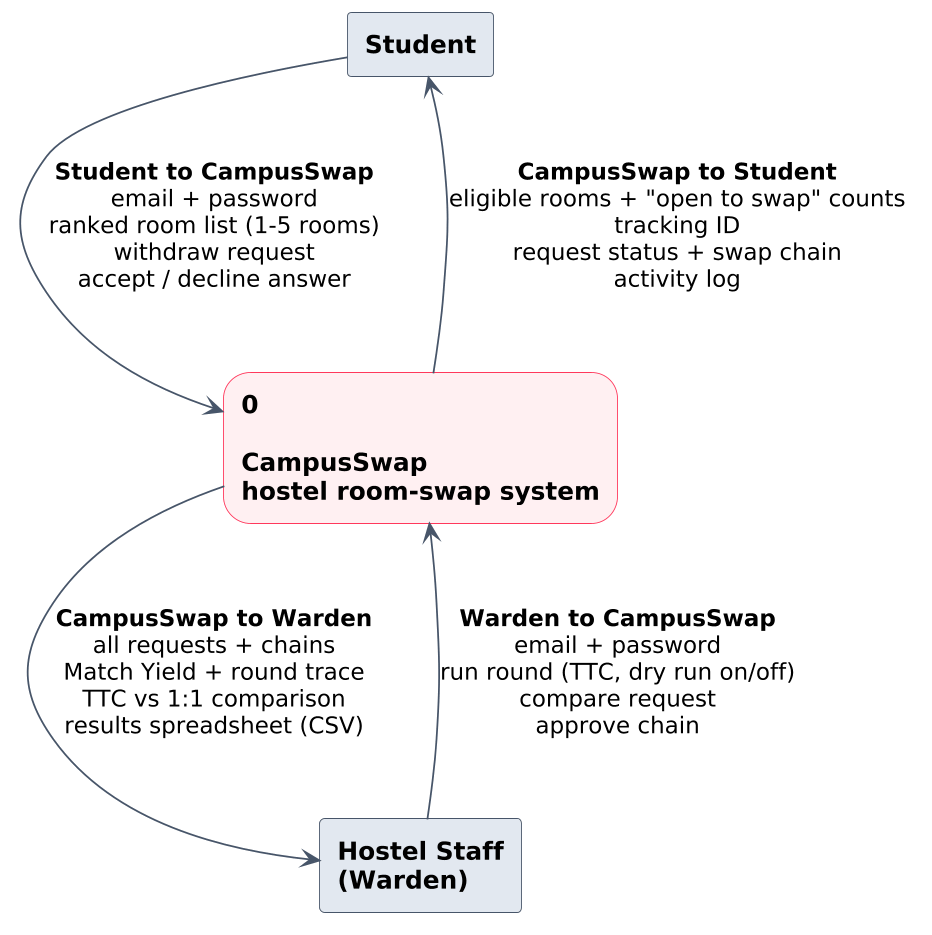
\includegraphics[width=\textwidth,height=0.4\textheight,keepaspectratio]{dfd-context.png}
  \caption[Data flow diagram, context level]{Data flow diagram, context
    level. Drawn before the final stage: it has no Faculty user and no
    outgoing email.}
  \label{fig:dfd0}
\end{figure}

\begin{figure}[H]
  \centering
  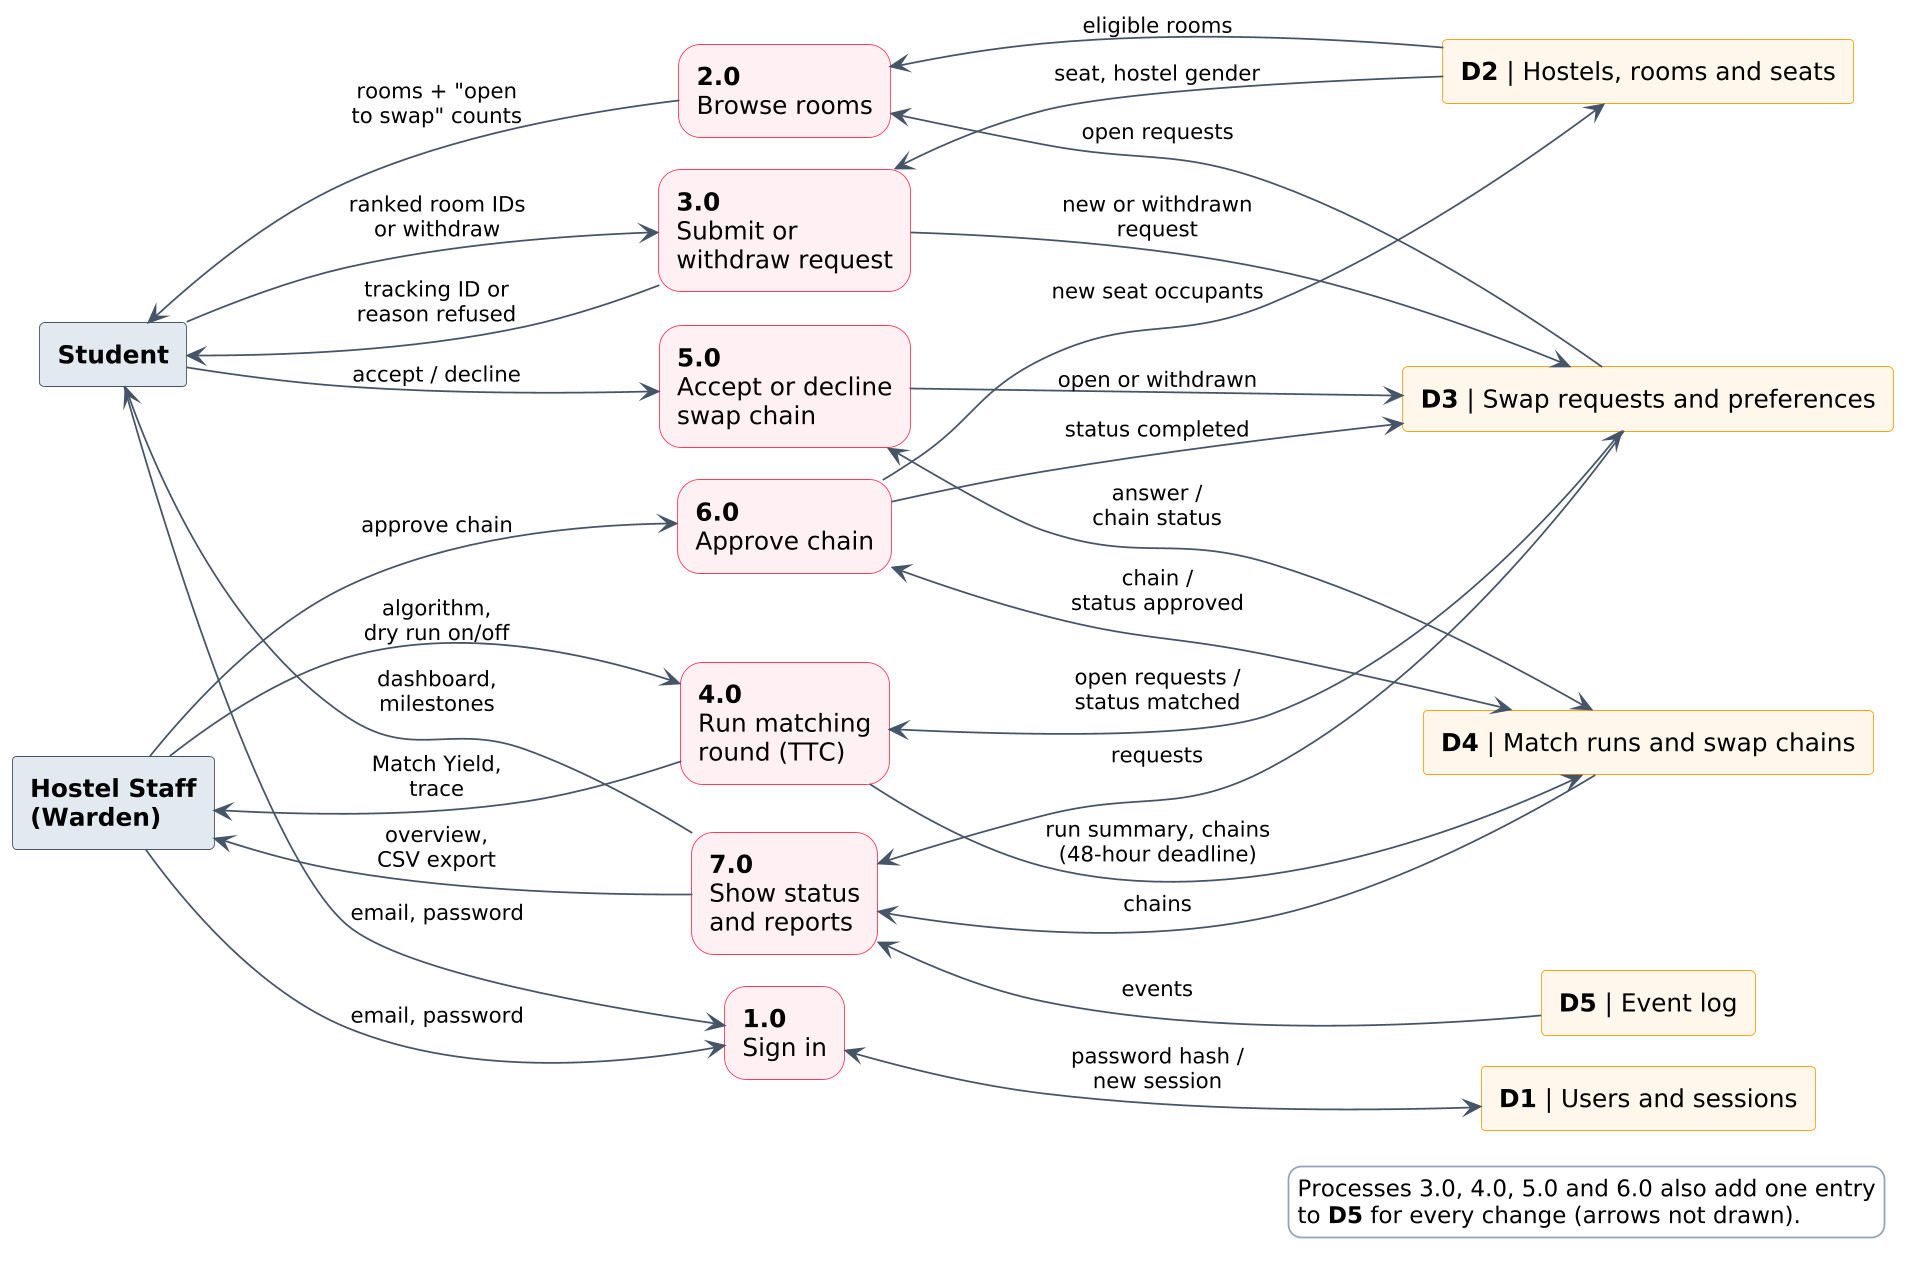
\includegraphics[width=\textwidth,height=0.75\textheight,keepaspectratio]{dfd-level1.png}
  \caption[Data flow diagram, level 1]{Data flow diagram, level 1. Drawn
    before the final stage: slot requests, the email outbox and the round
    timetable are not shown.}
  \label{fig:dfd1}
\end{figure}

\section{Data Model}

Figure~\ref{fig:class} shows the classes of the room part and
Figure~\ref{fig:er} the matching tables. The main decisions, unchanged
from the prototype, are:
\begin{itemize}
  \item \texttt{Student}, \texttt{Admin} and now \texttt{Faculty} are kinds
    of \texttt{User}, stored in one \texttt{users} table with a
    \texttt{role} column.
  \item A \texttt{Room} owns 1--3 \texttt{Seat}s (beds). The unit that is
    traded is a seat, because in a double room only one of the two
    students may move.
  \item A \texttt{SwapRequest} owns 1--5 \texttt{Preference}s. A
    \texttt{MatchRun} owns its \texttt{SwapCycle}s (chains), each with at
    least two \texttt{CycleMember}s.
\end{itemize}

\begin{figure}[H]
  \centering
  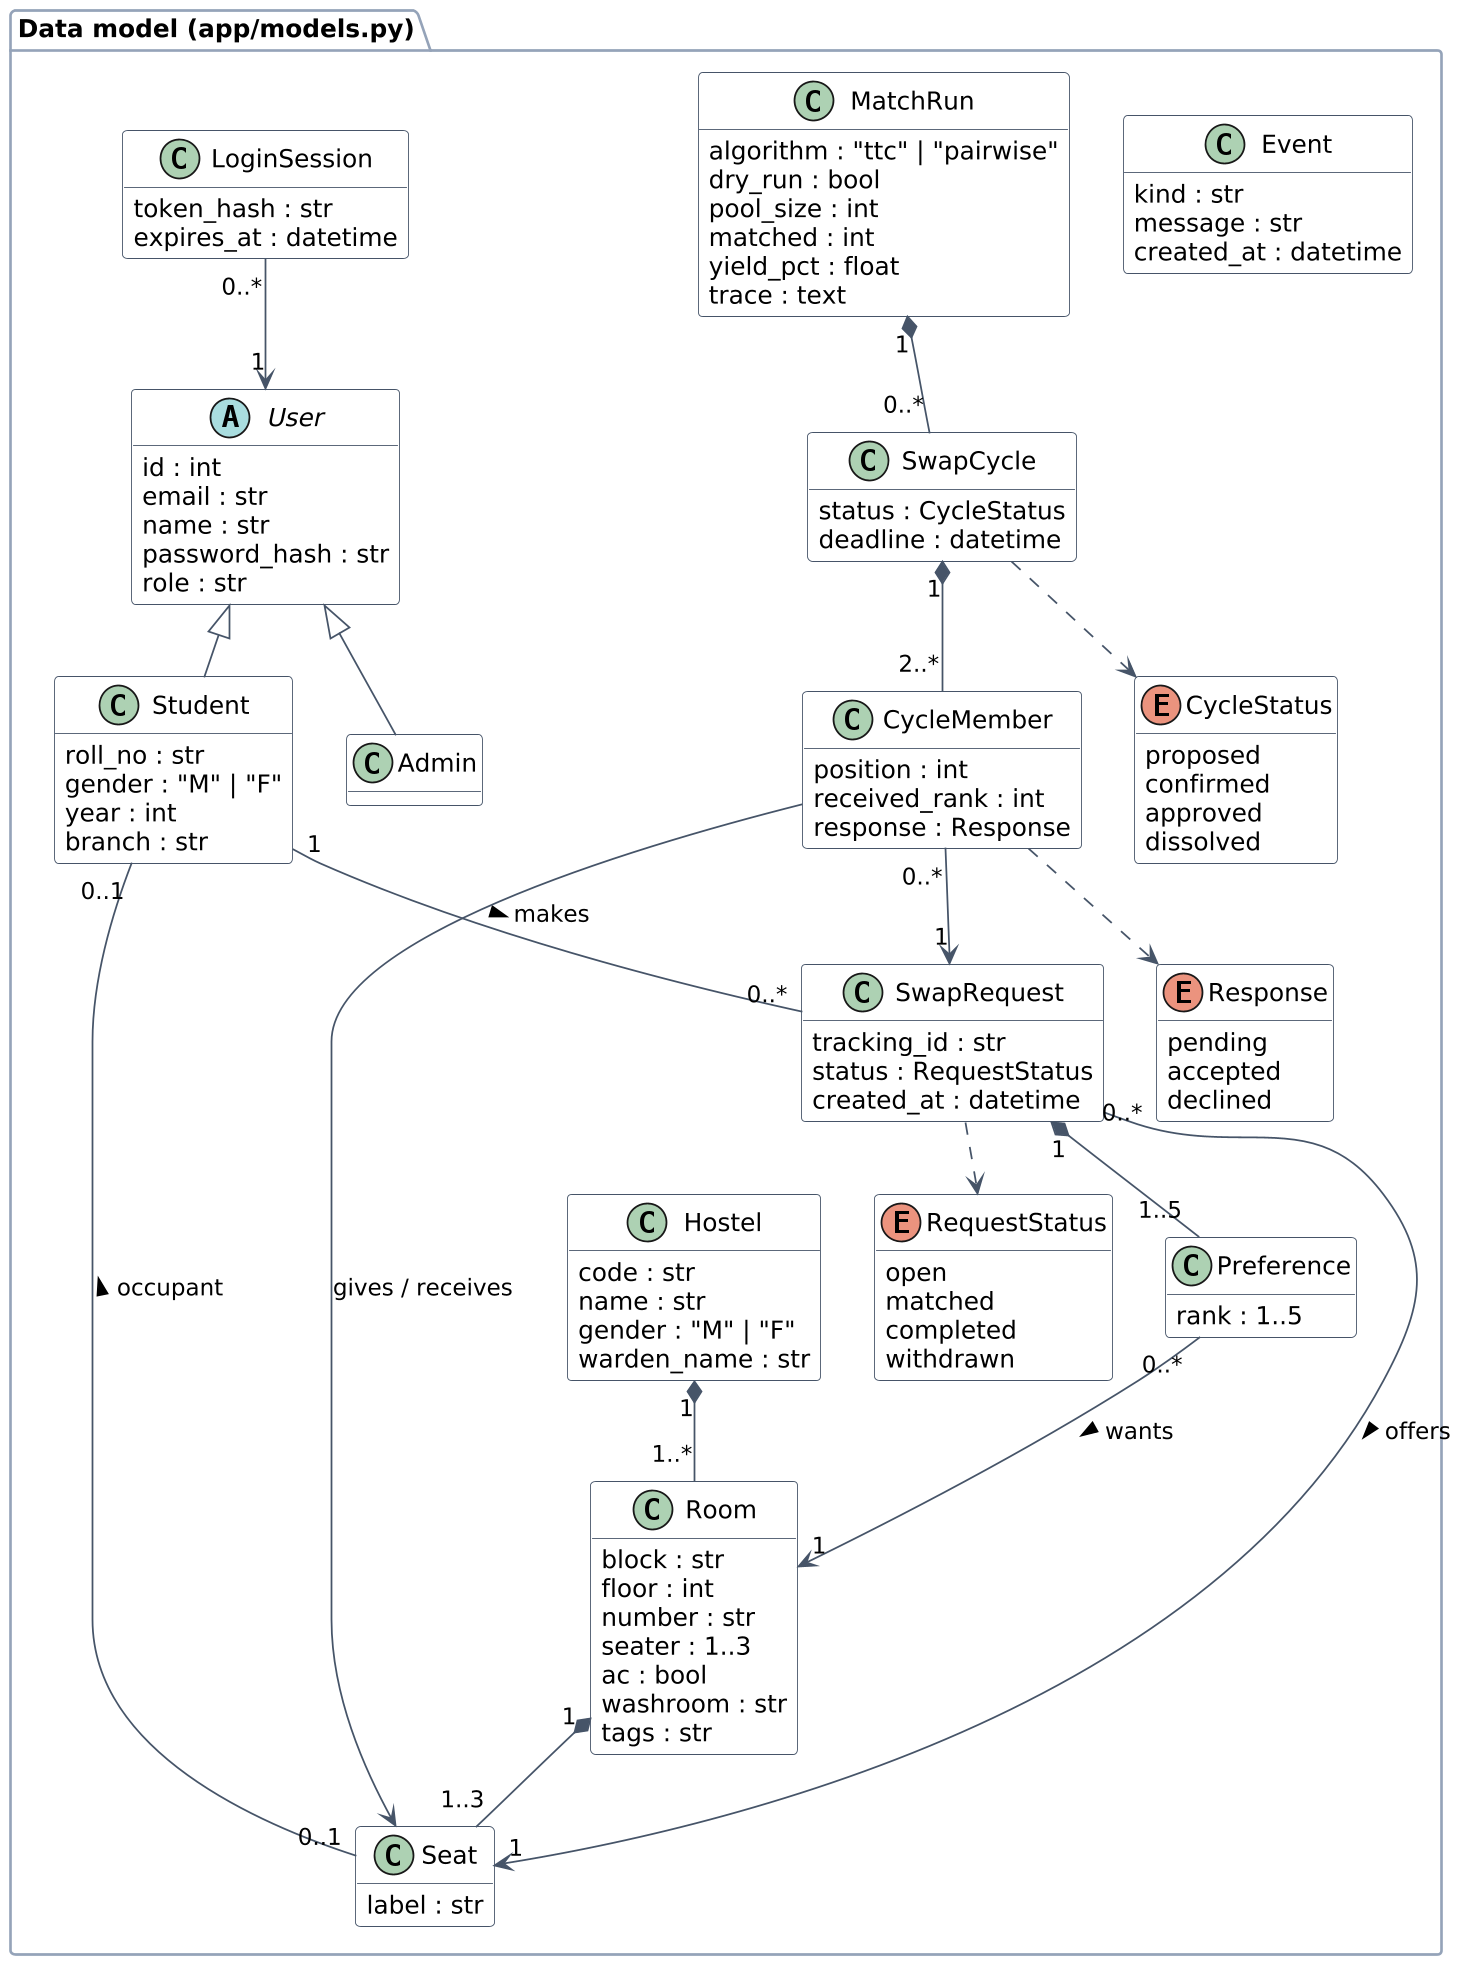
\includegraphics[width=\textwidth,height=0.8\textheight,keepaspectratio]{class.png}
  \caption[Class diagram, data model]{Class diagram of the data model.
    Drawn at the prototype stage: \texttt{Faculty}, the lecture-slot
    classes, \texttt{LoginFailure}, \texttt{Email} and \texttt{Schedule}
    are not shown (see Table~\ref{tab:newtables}).}
  \label{fig:class}
\end{figure}

\begin{figure}[H]
  \centering
  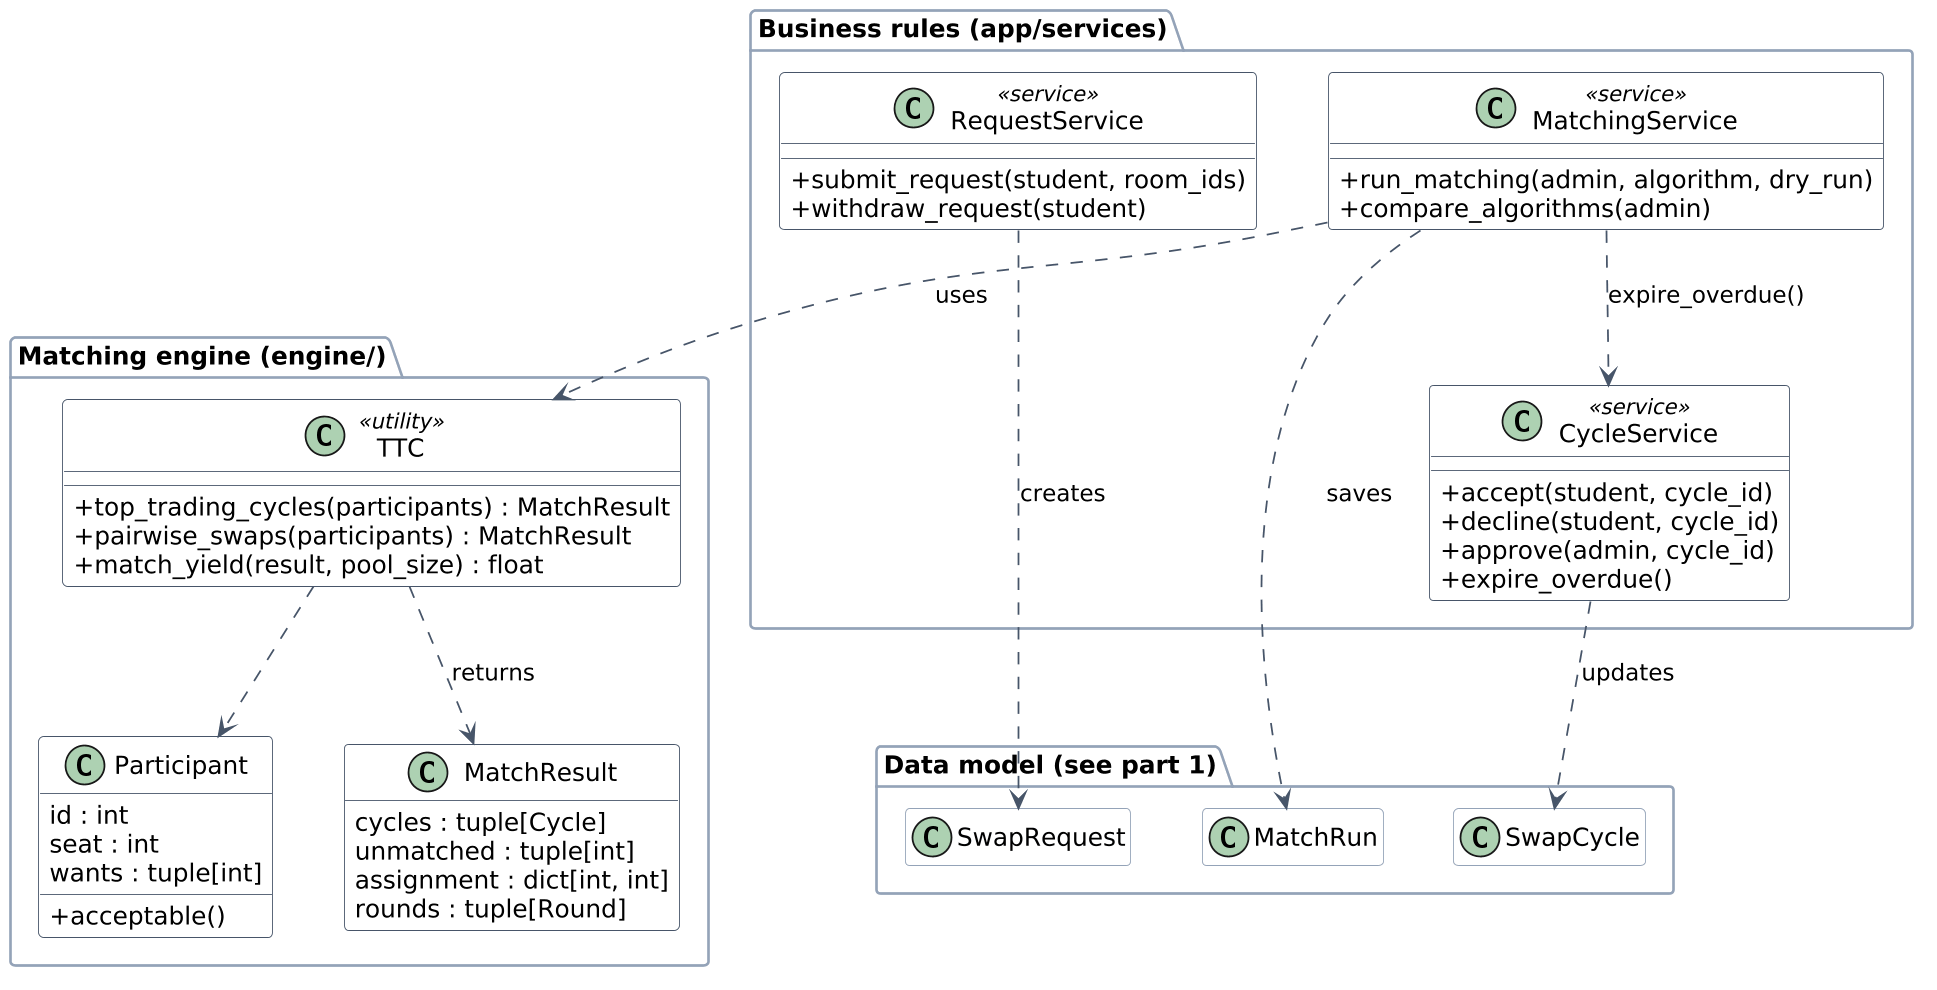
\includegraphics[width=\textwidth,height=0.8\textheight,keepaspectratio]{class-services.png}
  \caption[Class diagram, services and engine]{Class diagram of the
    services and the engine. Drawn at the prototype stage: the
    \texttt{signin}, \texttt{mail}, \texttt{schedule}, \texttt{pdf} and
    \texttt{slots} services are not shown.}
  \label{fig:classsvc}
\end{figure}

\begin{figure}[H]
  \centering
  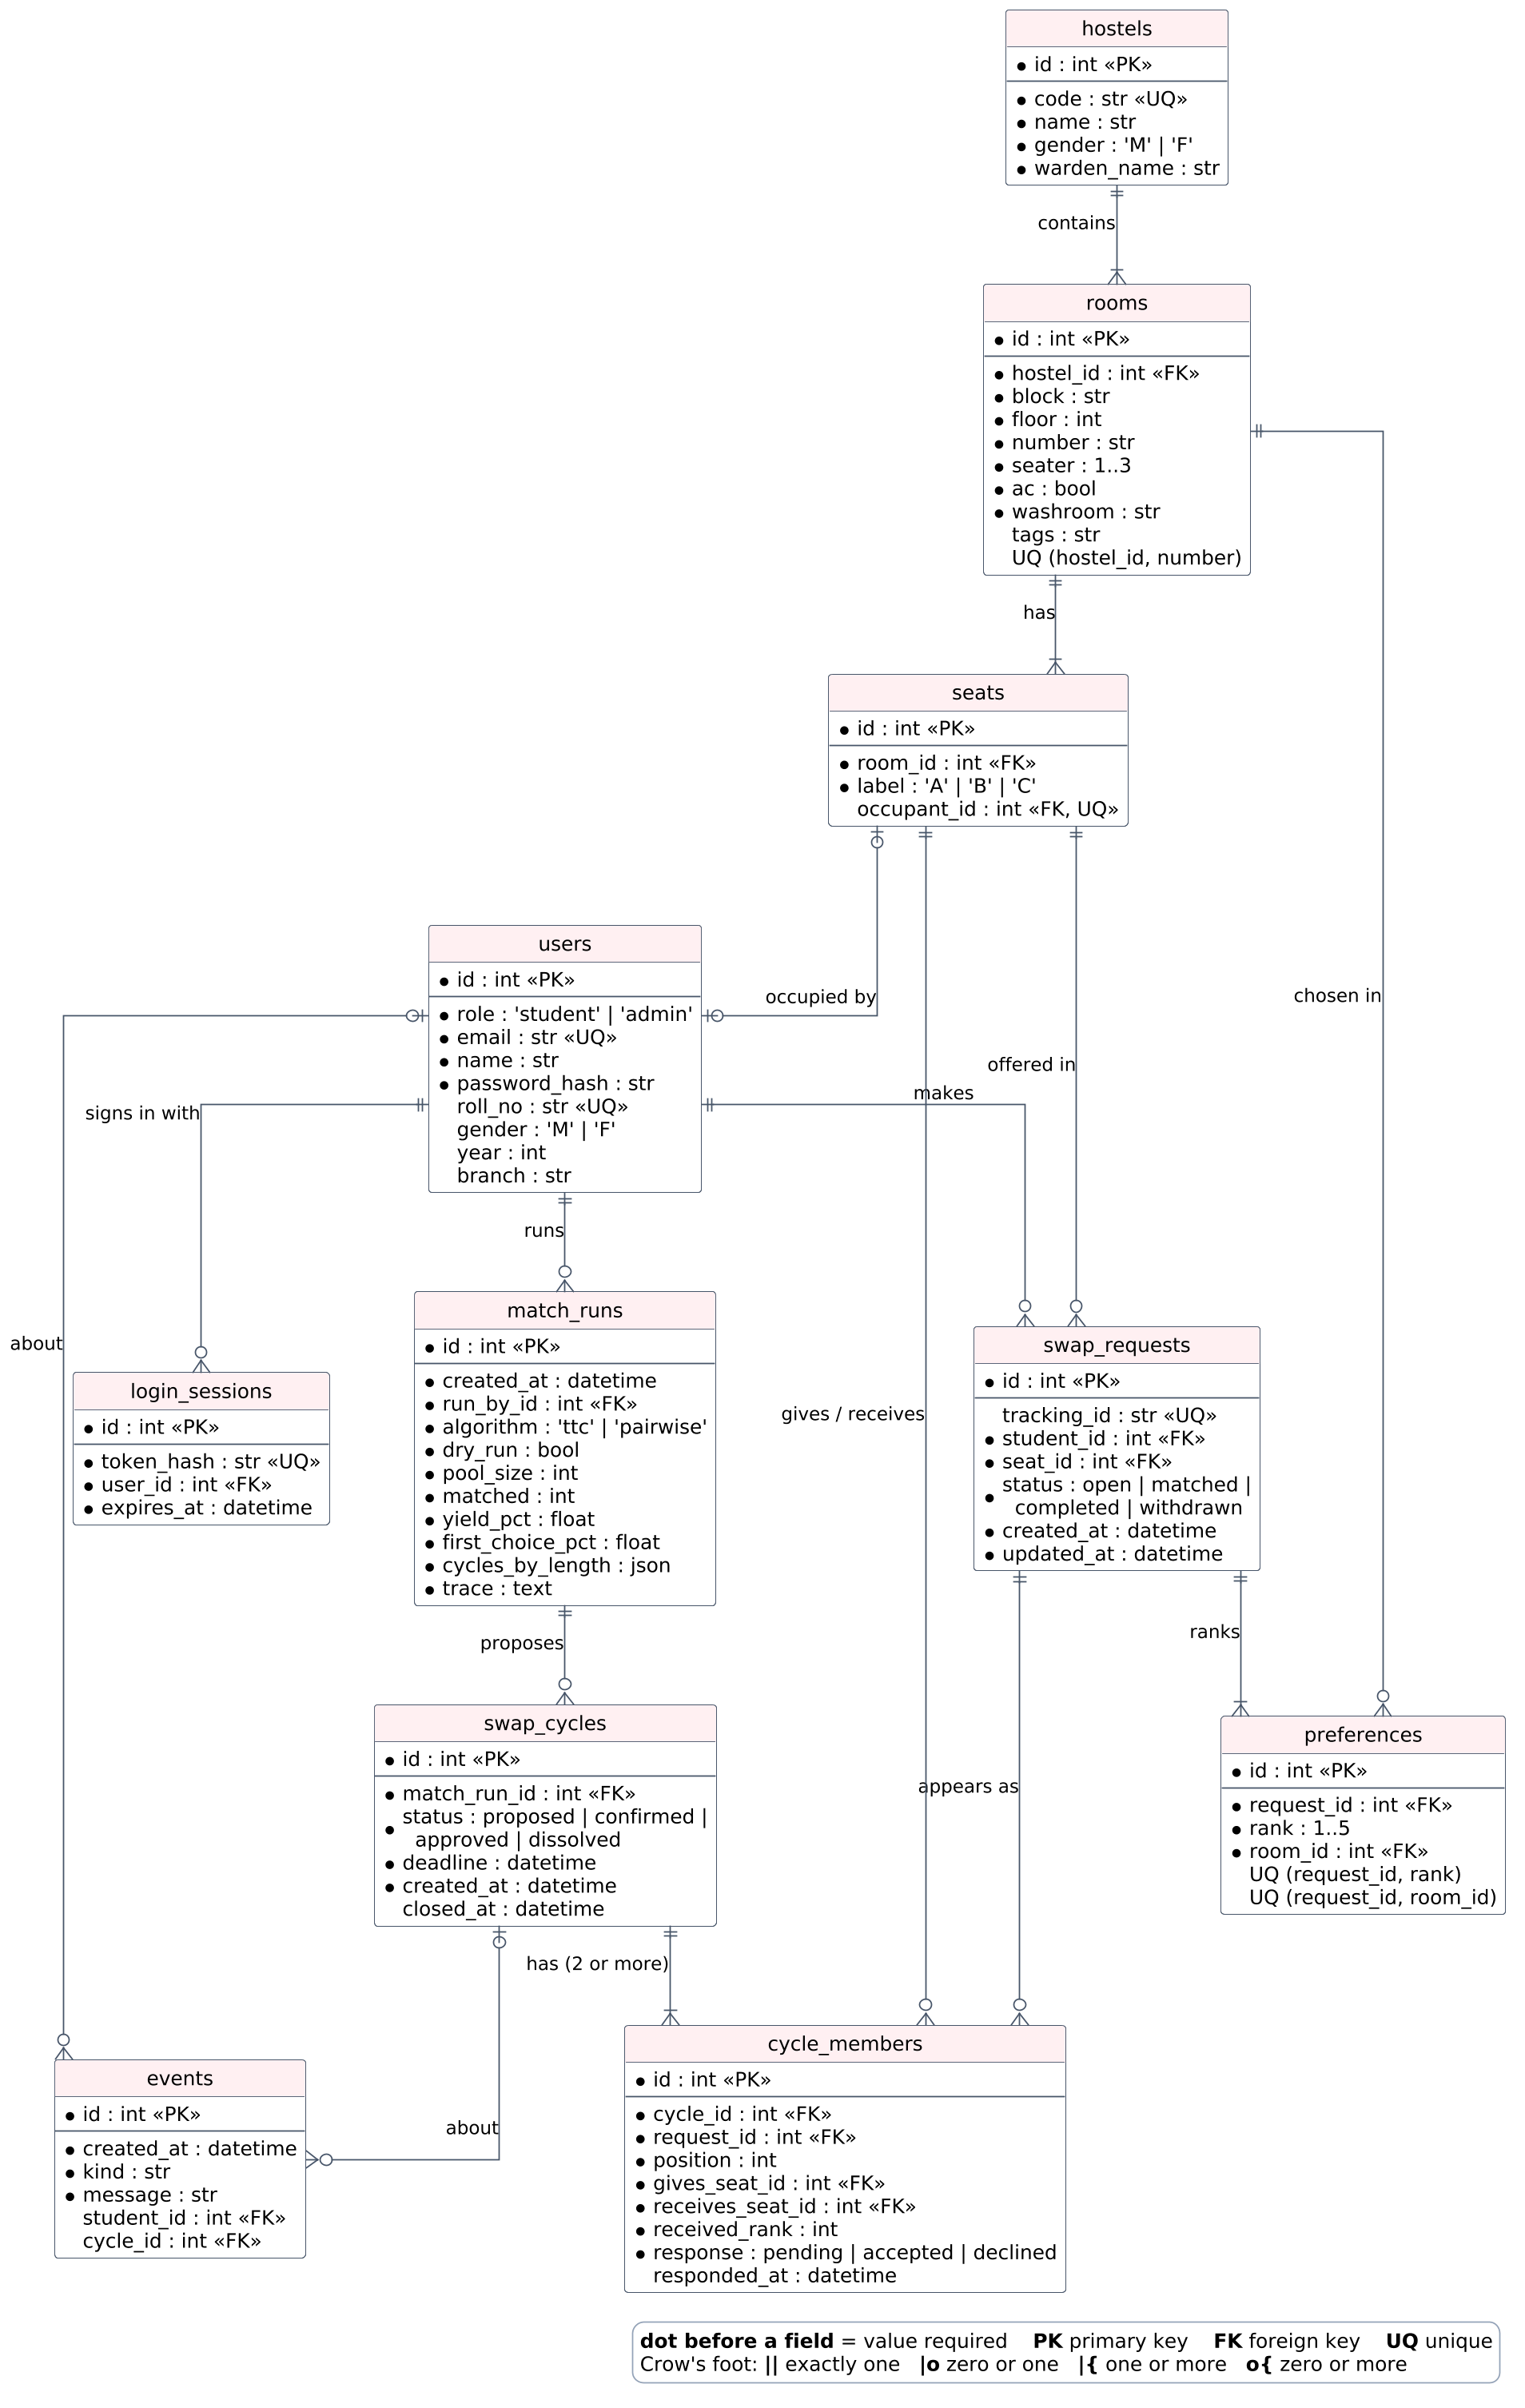
\includegraphics[width=\textwidth,height=0.8\textheight,keepaspectratio]{er.png}
  \caption[Entity relationship diagram]{Entity relationship diagram.
    Drawn before the final stage: it shows the eleven room tables only.
    The new tables and columns are listed in Table~\ref{tab:newtables}.}
  \label{fig:er}
\end{figure}

\begin{table}[H]
\centering
\small
\begin{tabularx}{\textwidth}{@{}lY@{}}
\toprule
\textbf{Table or column} & \textbf{What it holds} \\
\midrule
\texttt{login\_failures} & One row per failed sign-in: a key (the email, the network address, or both) and the time. Rows older than 15 minutes are deleted. \\
\texttt{emails} & The outbox: recipient, subject, body, status (\texttt{queued} or \texttt{sent}), number of attempts, last error, time sent. \\
\texttt{schedule} & One row: automatic rounds on or off, every how many hours, the next run time, who set it, the last run. \\
\texttt{lecture\_slots} & One weekly lecture: day, start minute, length (50 minutes), hall, course code and name, and the teacher who owns it. \\
\texttt{slot\_requests}, \texttt{slot\_preferences} & A teacher's offered slot and up to five ranked slots, with a tracking ID \texttt{SL-YYYY-NNNN}. \\
\texttt{slot\_cycles}, \texttt{slot\_cycle\_members} & Slot chains and their members, built like the room chains. \\
\midrule
\texttt{users.department} & The department of a faculty member. \\
\texttt{preferences.type\_*} & A choice may be a room type: \texttt{type\_hostel\_id} plus optional \texttt{type\_seater}, \texttt{type\_ac}, \texttt{type\_floor}; \texttt{room\_id} is then empty. \\
\texttt{swap\_cycles.approved\_by\_id} & Who approved the chain (printed on the approval form). \\
\texttt{cycle\_members.reminded\_at} & When the reminder email was queued, so it is sent only once. \\
\texttt{one\_active\_*} indexes & Database rules: at most one open or matched request per student, and per teacher. \\
\bottomrule
\end{tabularx}
\caption{Tables and columns added in the final stage.}
\label{tab:newtables}
\end{table}

\section{Matching Engine}
\label{sec:ttc}

\subsection{Model}

Each open request becomes a \emph{participant} $p$ that owns one item
$s_p$ (a seat, or a lecture slot) and has a ranked list $w_p$ of items it
would accept. Students rank rooms or room types; the room service turns
each choice into seats: a room gives its seats in seat-number order, and a
room type gives the seats of every matching room (except the student's
own) in room order. Teachers rank slots, which are used as they are. The
engine never sees rooms, slots or people, only numbers, which is why one
engine serves both features.

\subsection{Top Trading Cycles}

Algorithm~\ref{alg:ttc} is implemented in
\texttt{code/backend/engine/ttc.py}.

\begin{algorithm}[H]
\caption{Top Trading Cycles as implemented in CampusSwap}
\label{alg:ttc}
\begin{algorithmic}[1]
\Require participants $P$; each $p \in P$ owns item $s_p$ and ranks items $w_p$
\State $A \gets P$ \Comment{participants still in play}
\While{$A \neq \emptyset$}
  \For{each $p \in A$ whose current target has left}
    \State $\mathit{target}(p) \gets$ owner of the first item in $w_p$ still held in $A$, or $p$ itself
  \EndFor
  \State find every cycle in the graph $p \rightarrow \mathit{target}(p)$
  \For{each cycle $C$}
    \If{$|C| = 1$}
      \State the member keeps its own item (unmatched)
    \Else
      \State each $p \in C$ receives the item of $\mathit{target}(p)$
    \EndIf
    \State $A \gets A \setminus C$
  \EndFor
\EndWhile
\end{algorithmic}
\end{algorithm}

Because every participant points at exactly one participant, the pointer
graph always contains at least one cycle, so each round removes at least
one participant and the loop always ends. Cycles are searched in ID order
and each is rotated to start at its smallest ID, so the same pool always
gives the same result, whatever order the requests arrive in.

\textbf{Guarantees.} TTC never moves anyone to an item they ranked below
their own; no other outcome can make someone better off without making
someone worse off; no group can leave and do better by trading only among
themselves~\cite{shapley1974cores, roth1977weak}; and nobody gains by
ranking dishonestly~\cite{roth1982incentive}.

\textbf{Running time} (\Req{NFR-PERF-02}). Finding cycles visits each
remaining participant once per round, and there are at most $n$ rounds
for $n$ participants, so the cost is at most proportional to $n^2$. Each
pointer only moves forward through its own list, because an item that has
left never comes back, so all pointer moves together cost at most the
total length of all lists.

\subsection{Baseline and Metric}

To show what multi-way chains add, \texttt{pairwise\_swaps()} finds only
direct 1:1 swaps: two people are paired when each ranked the other's item,
best combined rank first, nobody in two pairs. It is only ever run as a
dry run. The result of a round is measured by the \emph{Match Yield}:
\[
  \mathrm{MY} = \frac{\text{people placed in a chain}}{\text{people in the pool}} \times 100.
\]

\section{Behaviour of a Room Swap}

Figure~\ref{fig:sequence} traces one room swap from request to approval
through every layer; Figure~\ref{fig:activity} shows the life of a request
with its decline and deadline branches.

\begin{figure}[H]
  \centering
  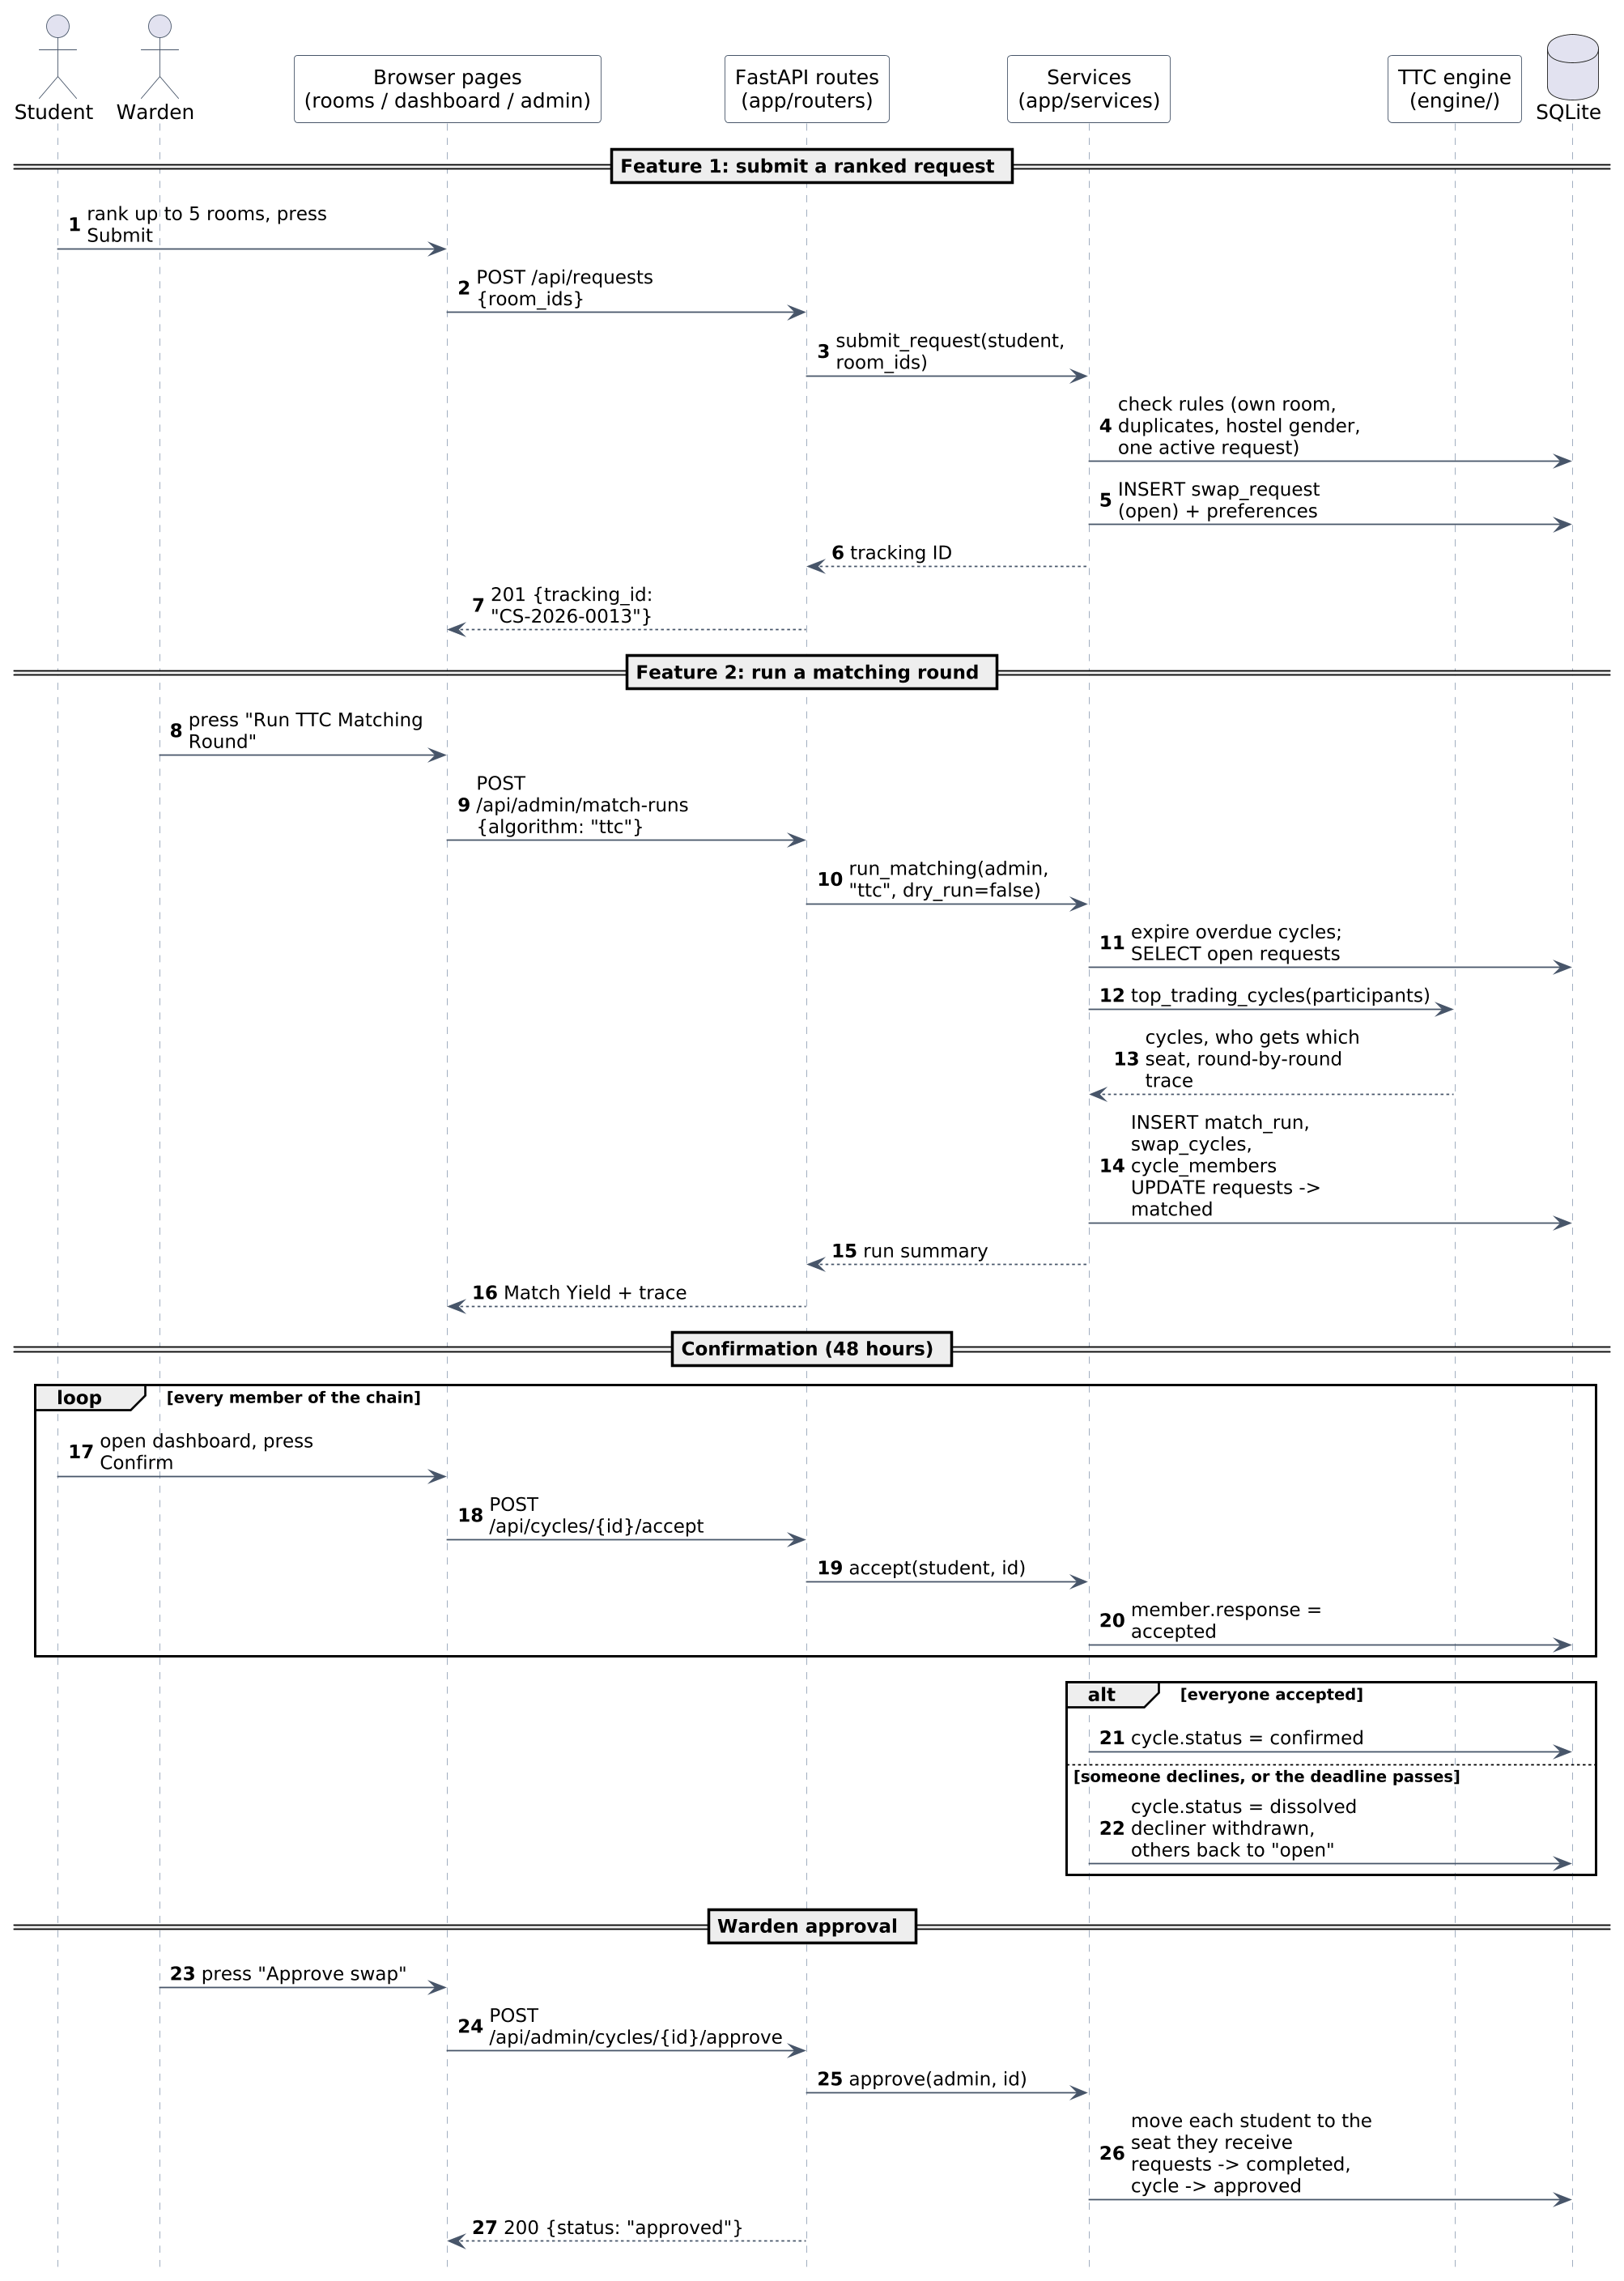
\includegraphics[width=\textwidth,height=0.8\textheight,keepaspectratio]{sequence.png}
  \caption[Sequence diagram]{Sequence diagram: submit, match, confirm and
    approve a room swap. Still accurate for these steps; the emails and
    the 30-second background check (Section~\ref{sec:tick}) are not shown.}
  \label{fig:sequence}
\end{figure}

\begin{figure}[H]
  \centering
  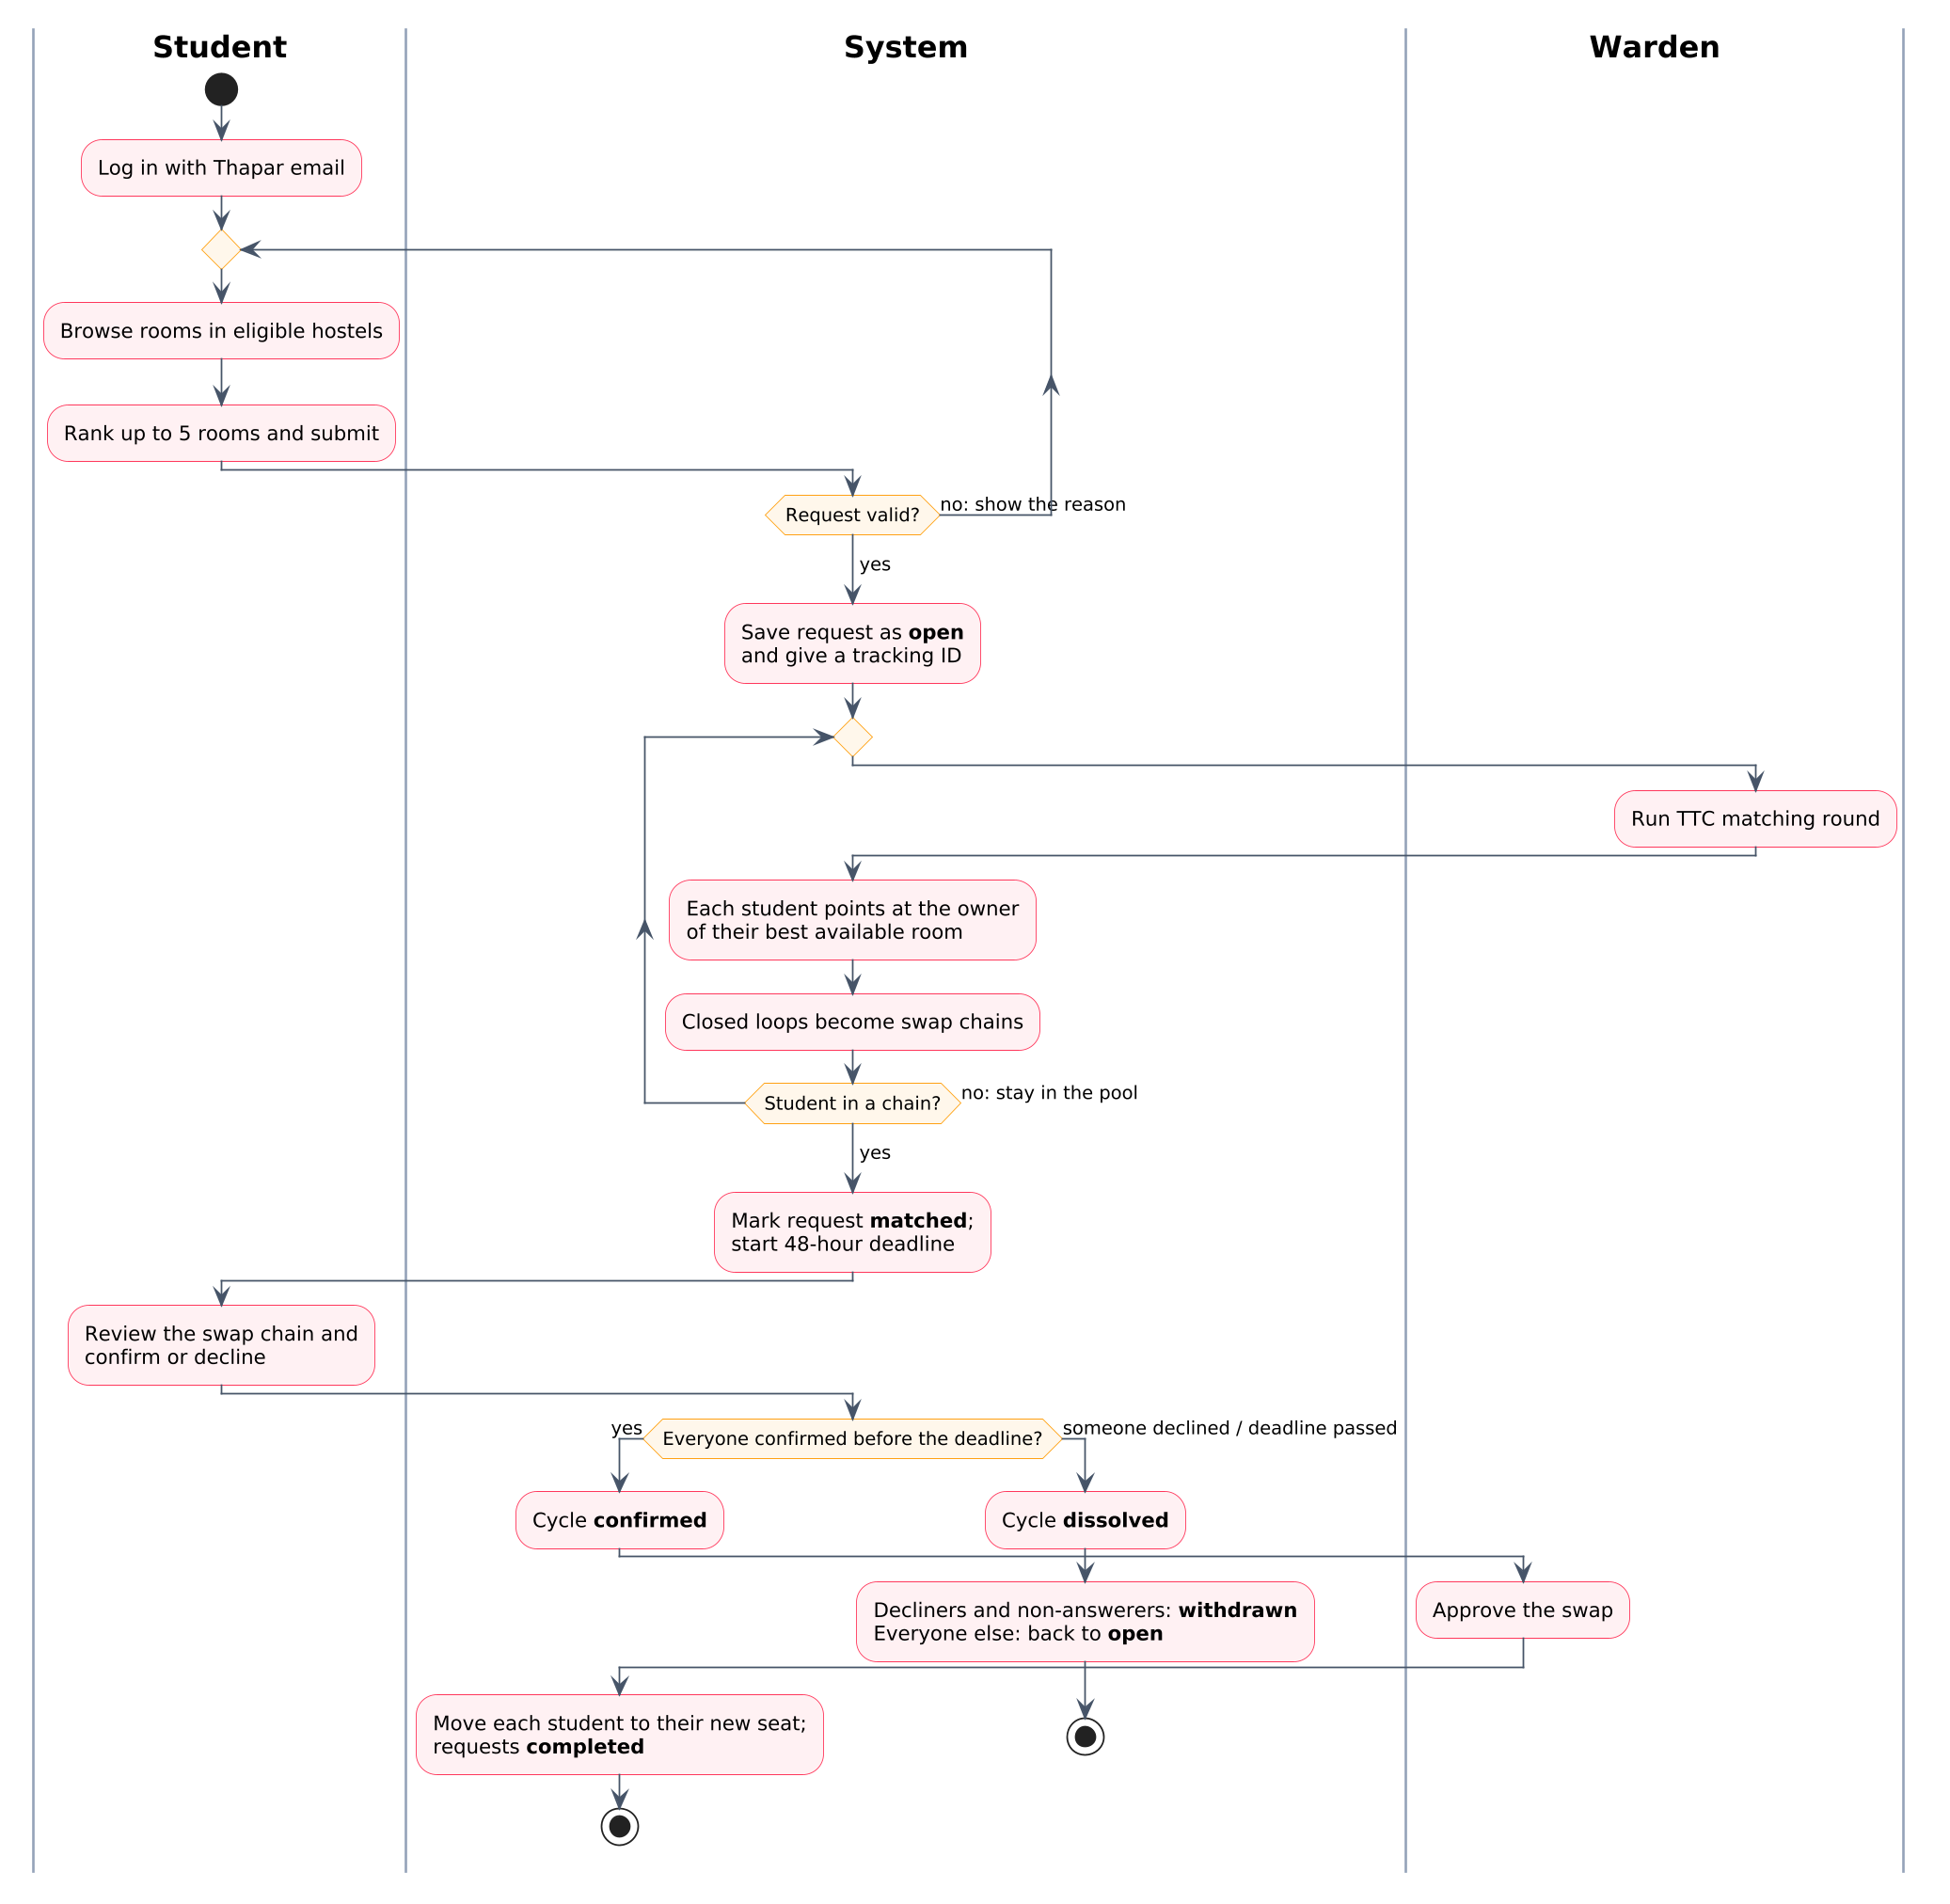
\includegraphics[width=\textwidth,height=0.8\textheight,keepaspectratio]{activity.png}
  \caption[Activity diagram]{Activity diagram: the life of a swap request.
    Drawn at the prototype stage: emails, room-type choices and automatic
    rounds are not shown.}
  \label{fig:activity}
\end{figure}

\section{Confirmation State Machine}

A \emph{state machine} is a fixed list of states something can be in, and
the events that move it from one state to another. Requests and chains
each have one (Figures~\ref{fig:streq} and~\ref{fig:stcyc}). Slot requests
and slot chains use exactly the same states.

\begin{table}[H]
\centering
\small
\begin{tabularx}{\textwidth}{@{}llY@{}}
\toprule
\textbf{From} & \textbf{To} & \textbf{When} \\
\midrule
-- & open & a valid ranked list is submitted \\
open & withdrawn & the owner withdraws \\
open & matched & a saved round places the request in a chain \\
matched & open & the chain is dissolved, but this member had not declined (and had answered, if the deadline passed) \\
matched & withdrawn & this member declined, or did not answer before the deadline \\
matched & completed & staff approve the confirmed chain \\
\bottomrule
\end{tabularx}
\caption{Status changes of a request (rooms and slots).}
\label{tab:reqstates}
\end{table}

\begin{table}[H]
\centering
\small
\begin{tabularx}{\textwidth}{@{}llY@{}}
\toprule
\textbf{From} & \textbf{To} & \textbf{When} \\
\midrule
-- & proposed & a saved round finds the chain; the deadline is 48 hours later \\
proposed & confirmed & the last pending member accepts \\
proposed & dissolved & any member declines, or the deadline passes \\
confirmed & approved & staff approve; the items change hands \\
confirmed & dissolved & slot chains only: at approval, a teacher no longer owns the slot they give (\texttt{stale\_swap}); everyone goes back to the pool \\
\bottomrule
\end{tabularx}
\caption{Status changes of a chain.}
\label{tab:cycstates}
\end{table}

\begin{figure}[H]
  \centering
  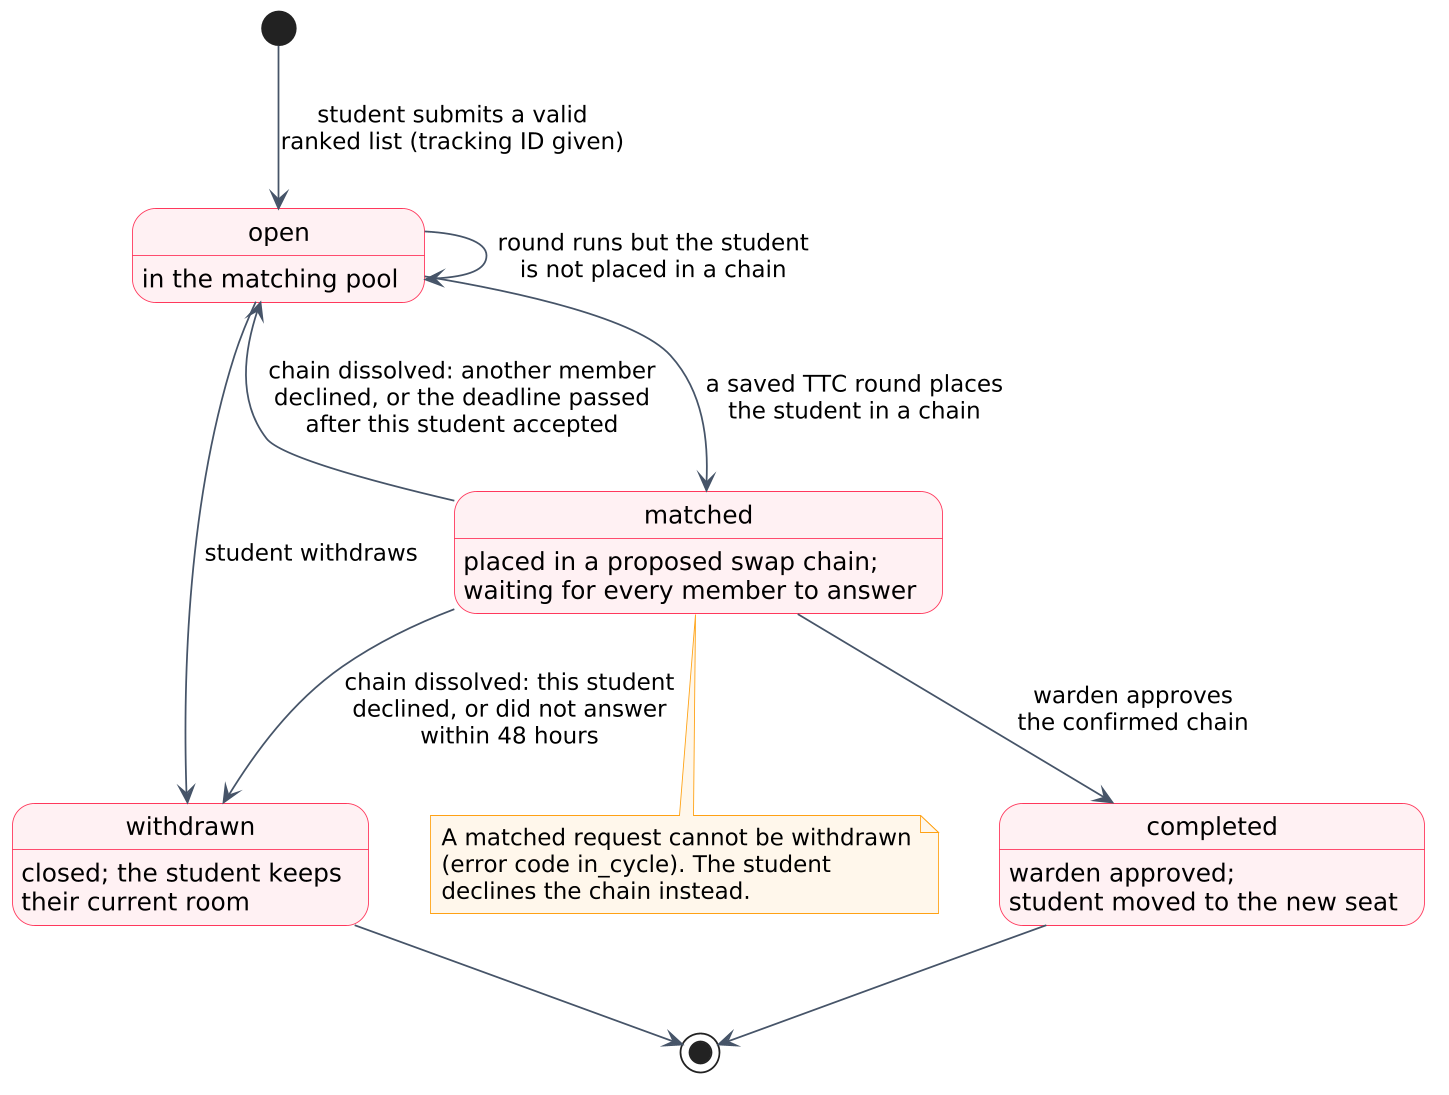
\includegraphics[width=\textwidth,height=0.6\textheight,keepaspectratio]{state-request.png}
  \caption{State diagram of a request.}
  \label{fig:streq}
\end{figure}

\begin{figure}[H]
  \centering
  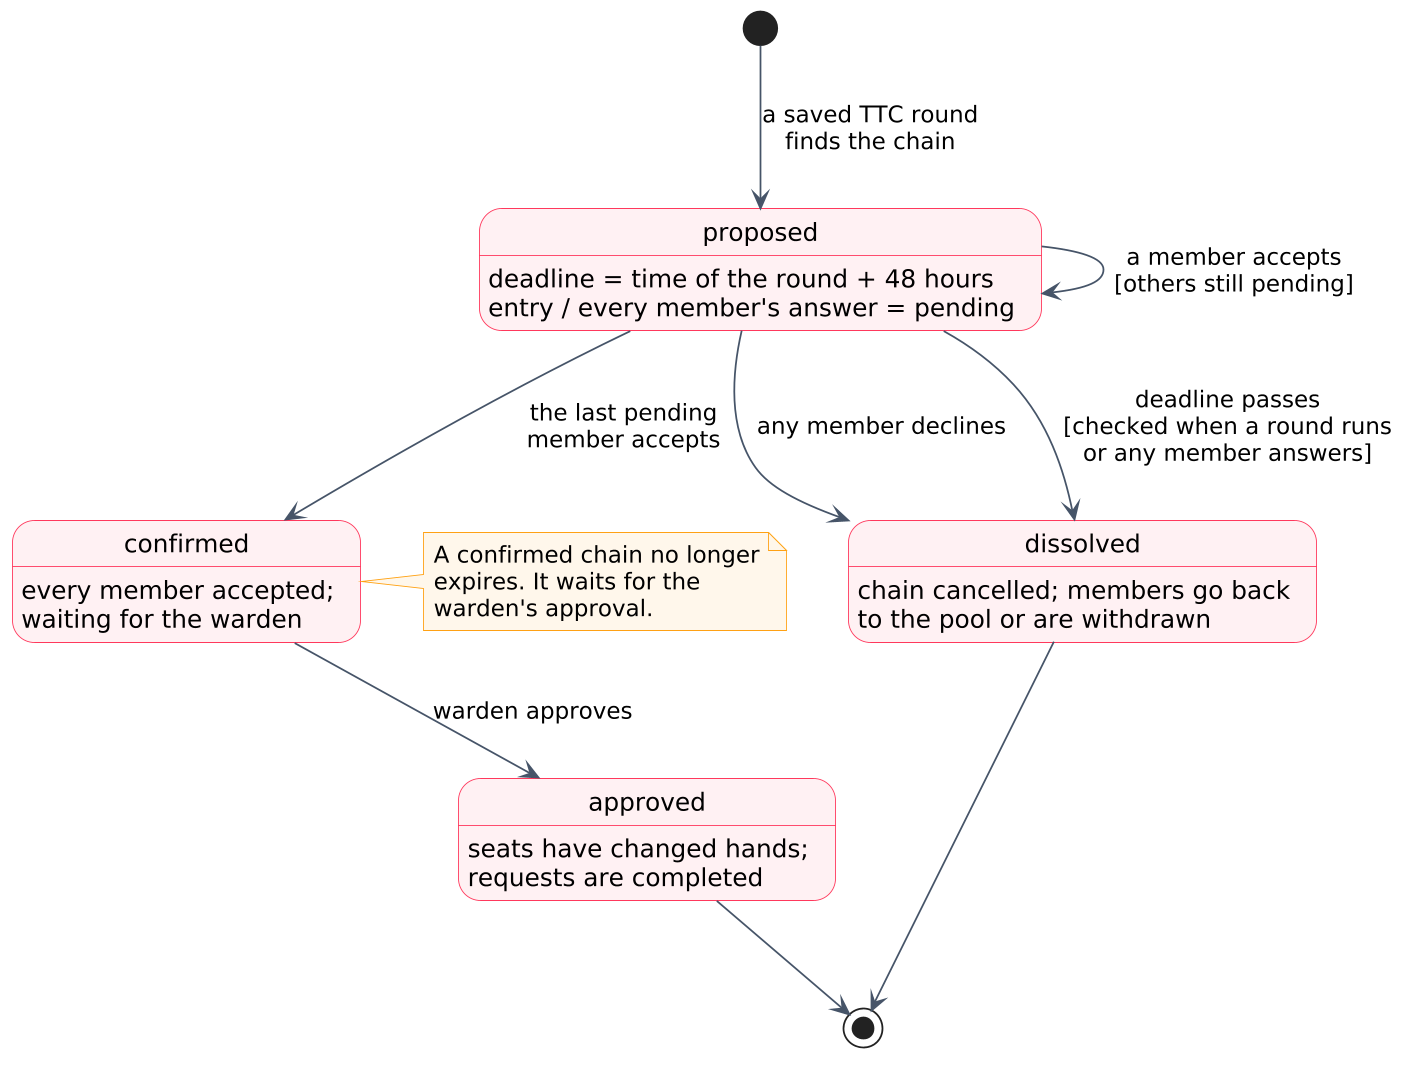
\includegraphics[width=\textwidth,height=0.6\textheight,keepaspectratio]{state-cycle.png}
  \caption[State diagram of a chain]{State diagram of a chain. Drawn
    before the final stage: the deadline is now also checked every 30
    seconds by the background check, and the slot-only
    \emph{confirmed $\rightarrow$ dissolved} step of
    Table~\ref{tab:cycstates} is not shown.}
  \label{fig:stcyc}
\end{figure}

\section{Background Jobs: the 30-Second Check}
\label{sec:tick}

In the prototype, an overdue chain was only dissolved when someone next
ran a round or answered. Emails, reminders and automatic rounds need
something that runs on its own, so the server now has one background job,
called the \emph{tick}. When the server is started with
\texttt{run.py}, it calls \texttt{schedule.tick()} every 30 seconds. One
tick, in this order:
\begin{enumerate}
  \item dissolves room chains and slot chains whose deadline has passed;
  \item queues a reminder for each room-chain member who has not answered,
    once 12 hours or less are left (one reminder per member);
  \item runs a saved TTC room round if the timetable says one is due;
  \item saves all of the above in one database transaction;
  \item only then hands queued emails to the mail server, if one is set up,
    one at a time, saving each result on its own. A slow mail server
    therefore never holds up a sign-in or a confirm.
\end{enumerate}
The tick runs in a separate thread so it never blocks a web page from
loading. If one tick fails, the error is written to the log and the next
tick tries again. In the tests the background job is switched off and the
tests call \texttt{tick()} directly with a chosen time, so no test has to
wait 30 seconds.

\textbf{Two things at the same moment.} Every database transaction first
takes SQLite's write lock (\texttt{BEGIN IMMEDIATE}). When an automatic
round and a staff member's Run click, or a last confirm and the deadline,
happen at the same moment, the second waits for the first and then reads
what it saved. Without this, the final review reproduced nine students
placed in two swaps at once; three tests in \texttt{test\_concurrency.py}
now guard against it. A request still waiting after five seconds gets a
plain ``busy, try again'' reply.

\textbf{Demo mode.} \texttt{run.py --demo} keeps every rule but shortens
the clock so a whole swap fits in a five-minute demonstration: 3 minutes
to confirm instead of 48 hours, the reminder 2 minutes before the deadline
instead of 12 hours, automatic rounds counted in minutes, and a tick every
5 seconds. The sign-in and staff pages say ``Demo mode'' while it is on.

\section{Sign-in Safety Design}
\label{sec:signin}

Three rules are checked by the server, in this order, before the password
is even looked at:
\begin{enumerate}
  \item \textbf{Institute address only.} The email is trimmed and turned
    to lower case; it must contain exactly one \texttt{@} and end in
    \texttt{@thapar.edu}, otherwise the answer is
    \texttt{400 not\_institute\_email}.
  \item \textbf{Failure limits.} Within any 15 minutes, the server counts
    failures in three ways and blocks further tries
    (\texttt{429 too\_many\_attempts}, with the number of minutes to wait)
    when one count is reached:
    \begin{itemize}
      \item 5 for one email \emph{from one network address} (stops one
        guesser);
      \item 20 from one network address for any emails (stops someone
        trying many accounts);
      \item 50 for one email from all addresses together (stops guessing
        spread over many addresses).
    \end{itemize}
    Because the 5-try limit is counted per address, a stranger who types
    wrong passwords for someone else's email does not lock the real owner
    out. A successful sign-in clears that email's failures.
  \item \textbf{Fair counting of network addresses.} With IPv6 (the newer
    form of internet address), one home or phone usually receives a whole
    block of addresses (a ``/64'' block), so a whole /64 block counts as one
    address. An IPv4 address written in IPv6 form is turned back into the
    IPv4 address, so different IPv4 users are not lumped together.
\end{enumerate}
For an unknown email the server still checks the password against a dummy
hash (a scrambled form of a password that cannot be turned back), so a
wrong email and a wrong password take about the same time and give the
same answer, \texttt{401 bad\_credentials}.

\textbf{HTTPS mode.} HTTPS is the encrypted form of the web protocol
HTTP. When the server is started with a certificate
(\texttt{run.py --cert cert.pem --key key.pem}) or with the setting
\texttt{CAMPUSSWAP\_SECURE=1}, three things change: plain HTTP requests
are redirected to HTTPS; the login cookie is marked \texttt{Secure}, so
the browser only sends it over HTTPS; and every answer carries the
\texttt{Strict-Transport-Security} header, which tells the browser to use
only HTTPS for this site for one year~\cite{rfc6797}. The mode is off by
default so the demo works on a laptop over plain HTTP.

\section{Lecture Slot Exchange Design}
\label{sec:slotdesign}

A \emph{lecture slot} is one weekly lecture: a day, a start time, a length
and a hall. The question was what moves in a swap. We decided:
\begin{itemize}
  \item \textbf{The teacher and the course move; the time and the hall
    stay.} If Dr.~A teaches UCS503 on Monday 08:00 in LT-101 and swaps with
    Dr.~B, then after approval Dr.~B's course is taught on Monday 08:00 in
    LT-101 by Dr.~B. Rooms and the timetable grid never change, only who
    teaches what in each cell. This matches how a department timetable is
    edited and means no hall can be double-booked by a swap.
  \item \textbf{Clash rule.} A teacher may not rank a slot that overlaps
    in time (same day, overlapping minutes) with any of their \emph{other}
    lectures. The slot being offered is left out of this check, because
    the teacher gives it up. A violation gives \texttt{400 slot\_clash}
    with the name of the clashing lecture, and the page shows such slots
    greyed out.
  \item \textbf{Same workflow as rooms.} One active request per teacher,
    up to five ranked slots, a separate slot round run by staff (by hand
    only; automatic rounds are for rooms), a 48-hour confirmation window,
    one email per member when a chain is found, and approval by staff.
  \item \textbf{Re-check at approval.} Between confirming and approving,
    the timetable could be changed by someone else. Approval therefore
    checks again that every member still owns the slot they give. If not,
    the chain is dissolved, nothing moves, and every member goes back to
    the pool (\texttt{409 stale\_swap}).
  \item \textbf{Safe moving.} All moves are read first and then applied,
    so no slot's course is overwritten before it has been copied to the
    next slot.
\end{itemize}

% =====================================================
\chapter{Implementation}
\label{ch:impl}
% =====================================================

\section{Technology Stack}

\begin{table}[H]
\centering
\small
\begin{tabularx}{\textwidth}{@{}lY@{}}
\toprule
\textbf{Layer} & \textbf{Technology} \\
\midrule
Pages & HTML, JavaScript modules, Tailwind CSS 3.4~\cite{tailwind} built on the team's machine; fonts and icons stored with the pages \\
Server & Python 3.12, FastAPI 0.141~\cite{fastapi}, Uvicorn 0.52 (the program that serves the app) \\
Database & SQLite through SQLAlchemy 2.0~\cite{sqlalchemy} \\
Approval form & fpdf2 2.8~\cite{fpdf2}, a library that draws PDF files from Python \\
Email & Python's built-in \texttt{smtplib} (SMTP is the standard way to hand mail to a mail server) \\
Testing & pytest 9~\cite{pytest}, FastAPI's \texttt{TestClient}, pypdf (to read the generated PDF back) \\
Diagrams & PlantUML~\cite{plantuml} \\
\bottomrule
\end{tabularx}
\caption{Technology stack.}
\end{table}

\section{Project Layout}

\begin{table}[H]
\centering
\small
\begin{tabularx}{\textwidth}{@{}lY@{}}
\toprule
\textbf{Folder or file} & \textbf{Contents} \\
\midrule
\texttt{code/backend/run.py} & Starts the server; \texttt{--reset} reloads fresh demo data; \texttt{--demo} shortens every wait to minutes; \texttt{--cert}/\texttt{--key} turn on HTTPS. Refuses to start on a database made by an older version. \\
\texttt{code/backend/seed.py} & The made-up demo data: four hostels, students in every bed, a staff account, eight teachers and sixteen lectures, and ready-made room and slot pools. \\
\texttt{code/backend/app/routers/} & The API: \texttt{auth}, \texttt{public}, \texttt{student}, \texttt{faculty}, \texttt{admin}. \\
\texttt{code/backend/app/services/} & The rules: \texttt{signin}, \texttt{requests}, \texttt{matching}, \texttt{cycles}, \texttt{mail}, \texttt{schedule}, \texttt{pdf}, \texttt{slots}, \texttt{views}, \texttt{events}. \\
\texttt{code/backend/app/models.py} & The database tables. \\
\texttt{code/backend/engine/} & TTC, the 1:1 comparison and the metrics. \\
\texttt{code/backend/tests/} & The automated tests, one file per area. \\
\texttt{code/frontend/public/} & The five pages, their scripts, styles, fonts and icons. \\
\bottomrule
\end{tabularx}
\caption{Where things are in the repository~\cite{campusswaprepo}.}
\end{table}

\section{New Features}

\subsection{Institute-only email and attempt limits}
The rules of Section~\ref{sec:signin} are in
\texttt{app/services/signin.py}. A failed sign-in writes one
\texttt{login\_failures} row per key and saves it at once, so the record is
kept even though the request itself is answered with an error. Old rows
are deleted each time the limits are checked, so the table stays small.

\subsection{HTTPS mode}
\texttt{create\_app(secure=...)} in \texttt{app/main.py} adds FastAPI's
HTTPS redirect and a small step that adds the
\texttt{Strict-Transport-Security} header to every answer. The sign-in and
sign-out routes set and clear the cookie with \texttt{secure} equal to the
same setting.

\subsection{Room-type choices}
The request body may now be a list of \emph{choices}, each either
\texttt{\{room\_id\}} or \texttt{\{type: \{hostel, seater, ac, floor\}\}}; the
old \texttt{room\_ids} list still works. A type in a hostel of the other
gender, an unknown hostel, the same type twice, or a type that matches no
room except the student's own is refused (\texttt{wrong\_hostel\_gender},
\texttt{unknown\_hostel}, \texttt{duplicate\_room}, \texttt{empty\_type}).
The type is shown in words, for example ``Any 1-seater AC room in Hostel M,
floor~1''. After a round, the \emph{received choice} is the first choice in
the list that matches the room received.

\subsection{Email outbox and reminders}
Every email is first written to the \texttt{emails} table (the
\emph{outbox}). It leaves only when a mail server is named in the settings
(\texttt{CAMPUSSWAP\_SMTP\_HOST}, port, user, password, sender). Delivery
uses an encrypted connection (STARTTLS); a failure is recorded with its
reason and retried at the next tick, up to five attempts. Without a mail
server, emails stay \emph{queued}, and the staff page says plainly that no
mail is being sent rather than pretending it was. Times in emails are given
in Indian Standard Time.

\subsection{Automatic rounds}
Staff choose ``every $N$ hours'' ($1 \le N \le 336$, that is up to two
weeks) on the staff page. The next run time is stored. When a tick finds a
round due, it moves the next run time forward by whole steps until it is in
the future, so rounds missed while the server was off are not run several
times in a row. If a round started by hand is running at that moment, the
automatic round waits for the next tick.

\subsection{Approval form PDF}
For an approved room chain, staff can download a one-page A4 form
(\texttt{GET /api/admin/cycles/\{id\}/approval.pdf}). It shows the swap
number and round, the chain length, when it was found and approved and by
whom, a table of members (name, roll number, tracking ID, room given up,
room moved to, choice received), the time each member confirmed, and a
signature line for each student and for the warden. For a chain that is
not approved the answer is \texttt{409 not\_approved}. The form exists for
room swaps only.

\subsection{Event log CSV}
\texttt{GET /api/admin/events.csv} downloads the whole audit log, oldest
first, with the columns \texttt{id}, \texttt{time\_utc}, \texttt{kind},
\texttt{message}, \texttt{student}, \texttt{roll\_no}, \texttt{cycle\_id}.
CSV (comma-separated values) is a plain-text table that opens in any
spreadsheet program. Events about teachers appear with an empty
\texttt{student} column, because that column is filled from student
records only.

\subsection{Faculty slot exchange}
\texttt{app/services/slots.py} implements Section~\ref{sec:slotdesign}.
Teachers use \texttt{slots.html} and the \texttt{/api/faculty/...} routes;
staff use the \emph{Slots} tab of the staff console and the
\texttt{/api/admin/slots}, \texttt{/api/admin/slot-runs} and
\texttt{/api/admin/slot-cycles/\{id\}/approve} routes. Slot rounds have
their own lock, so a slot round and a room round can run at the same time,
but never two slot rounds.

\subsection{One active request, enforced by the database}
The service already refused a second open request, but two submits that
arrived at the same moment could both pass that check before either was
saved. Now the database itself has a \emph{partial unique index}: a rule
that allows only one row per student whose status is \texttt{open} or
\texttt{matched}~\cite{sqlitepartial} (and the same per teacher for slot
requests). The insert is done inside a \emph{savepoint} (a point inside a
transaction that can be undone on its own); if the database refuses it,
the user gets the normal \texttt{409 already\_active} message.

\section{Screens}
\label{sec:screens}

Figures~\ref{fig:s-login} to~\ref{fig:s-form} show the finished pages.
Every number on them comes from the database; nothing is invented for
show.

\begin{figure}[H]
  \centering
  \screenshot[0.6\textheight]{screen-login.png}{\textwidth}
  \caption{Sign-in page with Student, Hostel Staff and Faculty tabs and
    live public numbers.}
  \label{fig:s-login}
\end{figure}

\begin{figure}[H]
  \centering
  \screenshot[0.8\textheight]{screen-rooms.png}{\textwidth}
  \caption{Explore Rooms: filters, room cards and the ranked list, which
    can hold rooms and room types.}
  \label{fig:s-rooms}
\end{figure}

\begin{figure}[H]
  \centering
  \screenshot[0.75\textheight]{screen-dashboard-ring.png}{\textwidth}
  \caption{Student dashboard: a proposed 4-way chain drawn as a ring, with
    each member's answer, the time left and the confirm and decline
    buttons.}
  \label{fig:s-ring}
\end{figure}

\begin{figure}[H]
  \centering
  \screenshot[0.8\textheight]{screen-admin.png}{\textwidth}
  \caption{Staff console: overview numbers, matching round results and
    the request table.}
  \label{fig:s-admin}
\end{figure}

\begin{figure}[H]
  \centering
  \screenshot[0.8\textheight]{screen-admin-panels.png}{\textwidth}
  \caption{Staff console: the step-by-step trace of a round, the automatic
    round timetable, and the email outbox, which says plainly that emails
    are queued because no mail server is set up.}
  \label{fig:s-panels}
\end{figure}

\begin{figure}[H]
  \centering
  \screenshot[0.8\textheight]{screen-admin-slots.png}{\textwidth}
  \caption{Staff console, Slots tab after a saved slot round: 3 of 4
    teachers placed in a 3-way chain, each row showing the slot given up
    and the slot received.}
  \label{fig:s-adminslots}
\end{figure}

\begin{figure}[H]
  \centering
  \screenshot[0.8\textheight]{screen-slots-builder.png}{\textwidth}
  \caption{Faculty page before a request: the teacher picks the lecture to
    move, then ranks slots in the weekly timetable. Their own lectures and
    a slot that clashes with one of them are greyed out.}
  \label{fig:s-slotsbuilder}
\end{figure}

\begin{figure}[H]
  \centering
  \screenshot[0.8\textheight]{screen-slots.png}{\textwidth}
  \caption{Faculty page after a slot round: a proposed 3-way slot swap,
    showing the slot now and after the swap, and each teacher's answer.}
  \label{fig:s-slots}
\end{figure}

\begin{figure}[H]
  \centering
  \begin{subfigure}[t]{0.23\textwidth}
    \centering
    \screenshot[0.5\textheight]{screen-login-mobile.png}{\linewidth}
    \caption{Sign in}
  \end{subfigure}\hfill
  \begin{subfigure}[t]{0.23\textwidth}
    \centering
    \screenshot[0.5\textheight]{screen-rooms-mobile.png}{\linewidth}
    \caption{Rooms}
  \end{subfigure}\hfill
  \begin{subfigure}[t]{0.23\textwidth}
    \centering
    \screenshot[0.5\textheight]{screen-dashboard-mobile.png}{\linewidth}
    \caption{Dashboard}
  \end{subfigure}\hfill
  \begin{subfigure}[t]{0.23\textwidth}
    \centering
    \screenshot[0.5\textheight]{screen-slots-mobile.png}{\linewidth}
    \caption{Slots}
  \end{subfigure}
  \caption{The pages on a phone (390 pixels wide).}
  \label{fig:s-mobile}
\end{figure}

\begin{figure}[H]
  \centering
  \screenshot[0.75\textheight]{approval-form.png}{0.8\textwidth}
  \caption{The approval form PDF for an approved 2-way room swap.}
  \label{fig:s-form}
\end{figure}

% =====================================================
\chapter{Testing}
\label{ch:test}
% =====================================================

\section{Strategy}

Tests are small programs that run the real code and check its answers.
We used three levels:
\begin{itemize}
  \item \textbf{Unit tests on the engine:} TTC, the 1:1 comparison and the
    metrics on hand-made pools, plus 50 random pools that must obey the
    guarantees of Section~\ref{sec:ttc}. No database is involved.
  \item \textbf{Service tests:} each business rule is called directly on
    a fresh in-memory database loaded with the demo data, and with a fixed
    clock, so deadlines and limits can be tested by moving the clock
    instead of waiting.
  \item \textbf{HTTP tests:} FastAPI's \texttt{TestClient} sends real web
    requests to the app (sign in, cookies, roles, error answers, the PDF
    download, a whole swap from request to approval).
\end{itemize}
Every final-stage requirement was built \emph{test first}: a test that
failed was written before the code that made it pass, and then the whole
suite was run again so that nothing older broke.

\section{How to Re-run}

From the repository root:
\begin{center}
\texttt{python project-report-final/tools/make\_test\_tables.py}
\end{center}
This runs the whole suite and rewrites the three files in
\texttt{project-report-final/generated/} from the result, so the tables in
this chapter and in Appendix~\ref{app:tests} can only say \emph{Pass} if the
test really passed.

\textbf{Result of the last run:} \TestsPassed{} of \TestsTotal{} automated
tests passed (\TestsFailed{} failed) in \TestsSeconds\,s on \TestsDate.
They are grouped into \CasesTotal{} test cases in
Table~\ref{tab:testcases}.

\section{Test Cases}

Each row of Table~\ref{tab:testcases} is one test case. The
\emph{Actual} and \emph{Result} columns are filled in from the test run, not
typed by hand. The line under each row names the automated tests that carry
it out.

\begin{landscape}
\footnotesize
\setlength{\tabcolsep}{3.5pt}
\setlength{\AutoByWidth}{\linewidth}
\begin{xltabular}{\linewidth}{@{}l L{2.3cm} Y Y Y L{1.7cm} l@{}}
\caption{Test cases, with results from the last test run (\TestsDate).}\label{tab:testcases}\\
\toprule
\textbf{ID} & \textbf{Requirement} & \textbf{Steps} & \textbf{Input} & \textbf{Expected} & \textbf{Actual} & \textbf{Result} \\
\midrule
\endfirsthead
\toprule
\textbf{ID} & \textbf{Requirement} & \textbf{Steps} & \textbf{Input} & \textbf{Expected} & \textbf{Actual} & \textbf{Result} \\
\midrule
\endhead
\endfoot
\endlastfoot
% The generated rows use \multicolumn{7}{@{}l}{...} for the "Automated by"
% line. An l column cannot wrap, so for these rows only it is swapped for a
% full-width wrapping column, and swapped back after the last row.
\noalign{\global\let\multicolumn\AutoByMulticolumn}
\InputRows{generated/testcases.tex}
\noalign{\global\let\multicolumn\OrigMulticolumn}
\end{xltabular}
\end{landscape}

\section{Checked by Hand}

Some behaviour exists only in the browser (layout, dragging, drawing the
ring), so it is checked by a person on the running pages.

{\small
\begin{xltabular}{\textwidth}{@{}l L{2.1cm} Y Y L{2.2cm}@{}}
\caption{Checks done by hand on the pages.}\label{tab:handchecks}\\
\toprule
\textbf{ID} & \textbf{Requirement} & \textbf{Steps} & \textbf{Expected} & \textbf{Result} \\
\midrule
\endfirsthead
\toprule
\textbf{ID} & \textbf{Requirement} & \textbf{Steps} & \textbf{Expected} & \textbf{Result} \\
\midrule
\endhead
\bottomrule
\endlastfoot
HC-01 & NFR-PERF-03 & Open the sign-in, rooms, dashboard, staff and slots pages in a window 390 pixels wide. & No page scrolls sideways; every button can be reached. & Pass (3 Nov 2026, Chrome at 390 and 375 pixels): no page wider than the window on any of the five pages. \\
\midrule
HC-02 & NFR-PERF-04 & Disconnect from the internet and reload each page. & Fonts, icons and styles still load, because all of them are served by the app. & Pass (3 Nov 2026, every outside address blocked): 0 requests left the app; both fonts and the icons loaded on all five pages. \\
\midrule
HC-03 & FR-REQ-02 & On the rooms page, rank three rooms, move one with the up and down buttons, remove one, then submit. & The order and rank numbers change at once; the saved request has the order shown. & Pass: the list went A-102, B-301, A-101; after moving A-101 up, A-102, A-101, B-301; after removing A-102, A-101, B-301. The saved request has A-101 as choice~1 and B-301 as choice~2. \\
\midrule
HC-04 & FR-CONF-01 & Sign in as a member of a 3-way chain and open the dashboard. & The ring shows every member, the room each gives, who has answered, the choice received and the time left. & Pass: the ring shows all three members, the room each gives up, ``Waiting'' for each, ``Your 1st choice'' and the time left (the same layout as Figure~\ref{fig:s-ring}). \\
\midrule
HC-05 & FR-AUTH-08, FR-AUTH-03, FR-AUTH-04, FR-AUTH-10 & Sign in with a non-institute address, a wrong password, the wrong tab, and after five wrong passwords. & The page shows a clear message for each case (institute email needed; wrong email or password; switch tabs; try again in $N$ minutes). & Pass: ``Use your Thapar email''; ``Wrong email or password''; ``Switched to the Hostel staff tab''; on the sixth try ``Too many tries \ldots{} Try again in 1 minute'' (demo mode). \\
\midrule
HC-06 & FR-SLOT-01 & Sign in as a teacher and look at a slot that overlaps another of their lectures. & The slot is greyed out and cannot be ranked, and the reason is shown. & Pass: 6 slots greyed out for faculty1, each with its reason, e.g.\ ``Clashes with your UCS414 lecture (Wed 14:00--14:50).'' \\
\end{xltabular}
}

% =====================================================
\chapter{Evaluation}
\label{ch:eval}
% =====================================================

% ---------------------------------------------------------------------
% Numbers in this chapter come from these commands, run from the
% repository root on 3 November 2026 (Python 3.12.10, Windows laptop).
%
% (1) Seeded pools, through the real services on an in-memory database
%     (dry runs, nothing saved). Run from the repository root:
%   .venv/Scripts/python -c "
%   import sys; sys.path.insert(0,'code/backend')
%   from app.main import create_app; from seed import seed
%   from app.models import Admin; from sqlalchemy import select
%   from app.services.matching import compare_algorithms; from app.services import slots
%   from app.clock import utcnow
%   app = create_app('sqlite://', frontend_dir=None)
%   with app.state.session_factory() as db:
%       seed(db); admin = db.scalar(select(Admin)); now = utcnow()
%       for r in (*compare_algorithms(db, admin, now), slots.run_round(db, admin, True, now)):
%           print(r.algorithm, r.pool_size, r.matched, r.yield_pct, r.first_choice_pct, r.cycles_by_length)
%   "
% Output (algorithm, pool, matched, yield %, first choice %, chains):
%   ttc 12 9 75.0 100.0 {'2': 1, '3': 1, '4': 1}
%   pairwise 12 2 16.7 100.0 {'2': 1}
%   slot_ttc 4 3 75.0 100.0 {'3': 1}
%
% (2) The same script, after first calling the request services for the three demo students
%     (student1 ranks Hostel M B-101, student2 A-201, student3 A-101) and
%     slots.submit() for faculty1 (UCS503 -> UCS301) and faculty2 (UCS301 -> UCS503):
%   ttc 15 12 80.0 ... {'2': 1, '3': 2, '4': 1}
%   pairwise 15 2 13.3 ... {'2': 1}
%   slot_ttc 6 5 83.3 ... {'2': 1, '3': 1}
%
% (3) Engine only: random pools as in tests/test_ttc.py::_random_pool
%     (seats 10, 20, ...; each participant ranks k other seats at random),
%     TTC timed with time.perf_counter, median of 5 runs, pool seed 7;
%     yields over 200 pools of 100 (seeds 0..199):
%   100 median ms 0.3 / 1000: 5.5 / 2000: 16.0 / 5000: 83.6
%   k 3 ttc mean 60.9 sd 5.6 min 45 max 77 pair mean 8.4 sd 3.9
%   k 5 ttc mean 75.2 sd 4.5 min 63 max 87 pair mean 21.6 sd 5.2
% ---------------------------------------------------------------------

\section{TTC Against Direct 1:1 Swaps on the Demo Data}

We ran the real matching services on a fresh in-memory copy of the demo
data, once as delivered and once after the live-demo users had submitted
their requests (three students who form a 3-way room chain, two teachers
who form a 2-way slot swap). Each run is a dry run, so nothing was saved.

\begin{table}[H]
\centering
\small
\begin{tabular}{@{}lrrrrl@{}}
\toprule
\textbf{Pool} & \textbf{Size} & \textbf{Method} & \textbf{Matched} & \textbf{MY} & \textbf{Chains} \\
\midrule
Rooms, as seeded & 12 & TTC & 9 & 75.0\% & one 2-way, one 3-way, one 4-way \\
                 & 12 & 1:1 only & 2 & 16.7\% & one 2-way \\
Rooms, with demo students & 15 & TTC & 12 & 80.0\% & one 2-way, two 3-way, one 4-way \\
                 & 15 & 1:1 only & 2 & 13.3\% & one 2-way \\
\midrule
Slots, as seeded & 4 & TTC & 3 & 75.0\% & one 3-way \\
Slots, with demo teachers & 6 & TTC & 5 & 83.3\% & one 2-way, one 3-way \\
\bottomrule
\end{tabular}
\caption{Match Yield (MY) on the demo pools (real output of the services).}
\label{tab:demoyield}
\end{table}

In the seeded room pool every matched student received their first
choice. Direct swaps find only the one 2-way swap; the 3-way and 4-way
chains are invisible to them. The demo pools were \emph{designed} to
contain these chains, so they show that the system finds them, not how
often they occur in real life.

\section{TTC Against 1:1 Swaps on Random Pools}

To get a less hand-made picture, we generated 200 random pools of 100
people, each owning one item and ranking $k$ other items chosen at random,
and ran the engine on them. These are the same settings as in the
prototype report, re-run on the final code, and the numbers came out the
same.

\begin{table}[H]
\centering
\small
\begin{tabular}{@{}lcc@{}}
\toprule
 & \textbf{3 choices each} & \textbf{5 choices each} \\
\midrule
TTC Match Yield, mean (standard deviation) & 60.9\% (5.6) & 75.2\% (4.5) \\
TTC Match Yield, lowest--highest & 45--77\% & 63--87\% \\
1:1 swaps only, mean (standard deviation) & 8.4\% (3.9) & 21.6\% (5.2) \\
\bottomrule
\end{tabular}
\caption{Match Yield on 200 random pools of 100 people.}
\label{tab:randyield}
\end{table}

TTC places three to seven times more people than direct swaps. Two
cautions apply. Random choices are a simplification: real students crowd
onto a few popular rooms, which would lower both numbers, so only a pilot
in a real hostel can give the true Match Yield. And TTC can produce long
chains, which are fragile because one decline cancels the whole chain.

\section{Performance}

\Req{NFR-PERF-01} asks for a pool of 2{,}000 requests to be matched in under
2 seconds. Test case TC-28 checks exactly that on every test run. We also
timed the engine directly (median of five runs, five choices each):

\begin{table}[H]
\centering
\small
\begin{tabular}{@{}rr@{}}
\toprule
\textbf{People in the pool} & \textbf{TTC time} \\
\midrule
100 & 0.3 ms \\
1{,}000 & 5.5 ms \\
2{,}000 & 16.0 ms \\
5{,}000 & 83.6 ms \\
\bottomrule
\end{tabular}
\caption{TTC running time (Python 3.12.10 on the team's Windows laptop).}
\label{tab:perf}
\end{table}

The 2{,}000-student pool takes 16~ms, about one hundredth of the limit.
The time grows faster than the pool size, as expected from
Section~\ref{sec:ttc}, but even 5{,}000 people take under a tenth of a
second. These timings cover the engine only; a saved round also writes
the chains, events and emails to the database, which we did not time
separately.

% =====================================================
\chapter{Conclusion and Future Work}
\label{ch:conc}
% =====================================================

\section{Summary}

CampusSwap now does everything the SRS asks except Microsoft single
sign-on. Students rank rooms or room types; teachers rank lecture slots;
one Top Trading Cycles engine finds multi-way chains for both; every member
confirms; staff approve, file a printed form, and keep a downloadable
record. Rounds can run on a timetable, members are emailed, and sign-in is
protected against password guessing. \TestsPassed{} of \TestsTotal{}
automated tests passed on the last run.

\section{Honest Limits}

\begin{itemize}
  \item \textbf{No single sign-on} (\Req{FR-AUTH-11}): it needs an
    application registration in Thapar's Microsoft tenant that only the
    institute can create (Section~\ref{sec:sso}).
  \item \textbf{Email was never sent through a real mail server.} The
    tests use a stand-in sender that records the messages, and one that
    always fails. The SMTP code itself has not been run against a real
    server, so settings such as the port or login could still need fixing
    on first use.
  \item \textbf{SQLite allows only one writer at a time.} That is enough
    for one campus, but many people saving at the same moment would wait
    for each other. The round locks are kept in the server's memory, so
    they only work while one server process runs. A larger deployment
    would need a database server such as PostgreSQL (the one-active-request
    rule is already written for it) and a shared lock.
  \item \textbf{No automated browser tests.} Page-only behaviour (layout
    on phones, dragging, the ring, the messages on the sign-in page) is
    checked by hand (Table~\ref{tab:handchecks}). A tool that drives a real
    browser would catch mistakes there automatically.
  \item \textbf{Some built rules have no test} (listed under
    Table~\ref{tab:status}).
  \item \textbf{Behind a proxy, sign-in limits would see one address.} The
    limits use the network address the server sees. If the app is put
    behind another server that forwards requests, every user would appear
    to come from that server's address, and the 20-per-address limit would
    then affect everyone together.
  \item \textbf{Not deployed.} The app runs on one laptop for the demo;
    HTTPS mode is ready but has not been used on a public server.
  \item \textbf{Made-up data only.} The Match Yield of a real hostel is
    still unknown.
\end{itemize}

\section{Future Work}

\begin{enumerate}
  \item Microsoft single sign-on, once the IT office registers the app.
  \item A pilot with 20--40 students from one hostel wing, to measure real
    Match Yield, time to approval and how often chains are declined.
  \item Handling long, fragile chains: a length limit, or re-running TTC on
    the remaining members after a decline.
  \item Browser tests for the page-only checks, and tests for the rules
    listed as having none.
  \item Deployment on an institute server with HTTPS and a real mail
    server.
\end{enumerate}

\section{Team Roles}

\begin{table}[H]
\centering
\small
\begin{tabularx}{\textwidth}{@{}lY@{}}
\toprule
\textbf{Role} & \textbf{Responsibility} \\
\midrule
P1 Frontend & the five pages, their scripts and the styling build \\
P2 Backend and sign-in & API routes, sessions, sign-in limits, request and confirmation rules, email and timetable \\
P3 Matching engine & TTC, the 1:1 comparison, Match Yield, the slot rounds and the engine tests \\
P4 Data, diagrams and delivery & data model, demo data, UML diagrams, the approval form, documentation and this report \\
\bottomrule
\end{tabularx}
\caption{Team roles.}
\end{table}

% =====================================================
\appendix
\chapter{All Automated Tests}
\label{app:tests}
% =====================================================

Every automated test in the suite, grouped by test file, with its running
time and result from the last run on \TestsDate{} (\TestsPassed{} of
\TestsTotal{} passed). This table is generated; see Chapter~\ref{ch:test}.

{\footnotesize
\begin{xltabular}{\textwidth}{@{}Y r l@{}}
\caption{Every automated test and its result.}\label{tab:alltests}\\
\toprule
\textbf{Test} & \textbf{Seconds} & \textbf{Result} \\
\midrule
\endfirsthead
\toprule
\textbf{Test} & \textbf{Seconds} & \textbf{Result} \\
\midrule
\endhead
\endfoot
\endlastfoot
\InputRows{generated/alltests.tex}
\end{xltabular}
}

% ===== BIBLIOGRAPHY =====

\printbibliography[heading=bibintoc]

\end{document}
